% Multumiri lui Gabriel Majeri, acest sablon a fost creat pe baza
% codului sursa a lucrarii sale de licenta. 
% Codul sursa: https://github.com/GabrielMajeri/bachelors-thesis
% Website: https://www.gabrielmajeri.ro/

\documentclass[12pt, a4paper]{report}

% Suport pentru diacritice și alte simboluri
\usepackage{fontspec}

% Suport pentru mai multe limbi
\usepackage{polyglossia}

\usepackage{longtable}

% Setează limba textului la engleza
\setdefaultlanguage{english}
% Am nevoie de romana pentru rezumat
\setotherlanguages{romanian}

% Indentează și primul paragraf al fiecărei noi secțiuni
\SetLanguageKeys{english}{indentfirst=true}

% Suport pentru diferite stiluri de ghilimele
\usepackage{csquotes}

\usepackage{multirow}
\usepackage{subcaption}

\DeclareQuoteStyle{english}
  {\quotedblbase}
  {\textquotedblright}
  {\guillemotleft}
  {\guillemotright}

% Utilizează biblatex pentru referințe bibliografice
\usepackage[
    maxbibnames=50,
    sorting=none
]{biblatex}

\addbibresource{bibliography.bib}

% Setează spațiere inter-linie la 1.5
\usepackage{setspace}
\onehalfspacing

% Modificarea geometriei paginii
\usepackage{geometry}

% Include funcțiile de grafică
\usepackage{graphicx}
% Încarcă imaginile din directorul `images`
\graphicspath{{./images/}}

% Listări de cod
\usepackage{listings}
% Color package for listings
\usepackage{xcolor}
% GitHub color palette
\definecolor{github_background}{HTML}{ffffff}
\definecolor{github_foreground}{HTML}{24292e}
\definecolor{github_keyword}{HTML}{d73a49}
\definecolor{github_string}{HTML}{032f62}
\definecolor{github_comment}{HTML}{6a737d}
\definecolor{github_number}{HTML}{005cc5}
\definecolor{github_function}{HTML}{6f42c1}

\lstset{
    language=Python,
    basicstyle=\ttfamily\small\color{github_foreground},
    keywordstyle=\color{github_keyword},
    stringstyle=\color{github_string},
    commentstyle=\color{github_comment},
    numberstyle=\tiny\color{github_number},
    identifierstyle=\color{github_function},
    backgroundcolor=\color{github_background},
    showspaces=false,
    showstringspaces=false,
    breaklines=true,
    frame=single,
    tabsize=4,
    captionpos=b,
    breakatwhitespace=false,
    escapeinside={\%*}{*)},
    numbers=left,
}

% Linkuri interactive în PDF
\usepackage[
    colorlinks,
    linkcolor={black},
    menucolor={black},
    citecolor={black},
    urlcolor={blue}
]{hyperref}

% Simboluri matematice codificate Unicode
\usepackage[warnings-off={mathtools-colon,mathtools-overbracket}]{unicode-math}

% Comenzi matematice
\usepackage{amsmath}
\usepackage{mathtools}

\usepackage{float}
\floatstyle{plain}
\newfloat{listing}{H}{lop}
\floatname{listing}{Listing}

% Formule matematice
\newcommand{\bigO}[1]{\symcal{O}\left(#1\right)}
\DeclarePairedDelimiter\abs{\lvert}{\rvert}

% Suport pentru rezumat în două limbi
% Bazat pe https://tex.stackexchange.com/a/70818
\newenvironment{abstractpage}
  {\cleardoublepage\vspace*{\fill}\thispagestyle{empty}}
  {\vfill\cleardoublepage}
\renewenvironment{abstract}[1]
  {\bigskip\selectlanguage{#1}%
   \begin{center}\bfseries\abstractname\end{center}}
  {\par\bigskip}

% Suport pentru anexe
\usepackage{appendix}

% Stiluri diferite de headere și footere
\usepackage{fancyhdr}

% Metadate
\title{Car Price Predictor Based on Machine Learning}
\author{Huțan Mihai-Alexandru}

% Generează variabilele cu @
\makeatletter

\begin{document}

% Front matter
\cleardoublepage
\let\ps@plain

% Pagina de titlu
\begin{titlepage}

% Redu marginile
\newgeometry{left=2cm,right=2cm,bottom=1cm}

\begin{figure}[!htb]
    \centering
    \begin{minipage}{0.2\textwidth}
        
\includegraphics[width=\linewidth]{logo-ub.png}
    \end{minipage}
    \begin{minipage}{0.5\textwidth}
        \large
        \vspace{0.2cm}
        \begin{center}
            \textbf{UNIVERSITY OF BUCHAREST}
        \end{center}
        \vspace{0.3cm}
        \begin{center}
            \textbf{
                FACULTY OF \\
                MATHEMATICS \\
                AND \\
                COMPUTER SCIENCE
            }
        \end{center}
    \end{minipage}
    \begin{minipage}{0.2\textwidth}
        
\includegraphics[width=\linewidth]{logo-fmi.png}
    \end{minipage}
\end{figure}

\begin{center}
\textbf{COMPUTER SCIENCE SPECIALIZATION}
\end{center}

\vspace{1cm}

\begin{center}
\Large \textbf{Bachelor thesis}
\end{center}

\begin{center}
\huge \textbf{\MakeUppercase{\@title}}
\end{center}

\vspace{3cm}

\begin{center}
\large \textbf{Student \\ \@author}
\end{center}

\vspace{0.25cm}

\begin{center}
\large \textbf{Thesis Coordinator \\ Prof. Dr. Ionescu Radu Tudor}
\end{center}

\vspace{2cm}

\begin{center}
\Large \textbf{Bucharest, June 2024}
\end{center}
\end{titlepage}
\restoregeometry
\newgeometry{
    margin=2.5cm
}

\fancypagestyle{main}{
  \fancyhf{}
  \renewcommand\headrulewidth{0pt}
  \fancyhead[C]{}
  \fancyfoot[C]{\thepage}
}

\addtocounter{page}{1}

% Rezumatul
\begin{abstractpage}


\begin{abstract}{english}

The second-hand car market in Romania is continually growing, registering over 660.000 transactions in 2023, according to data from Autovit \cite{autovit_statistics}. However, the market expansion is shadowed by challenges, particularly the inflated prices of used cars. In response to these market dynamics, this thesis introduces a web application under the brand \textit{RoCar}, tailored for the Romanian automotive market, designed to predict vehicle prices.

\textit{RoCar} utilizes a model specialized in Romania's economy and pricing, trained on data we have independently scraped. The application differentiates itself from other similar options by using not only structured data such as the year of production, manufacturer, model, and various options but also information extracted from images and descriptions, leveraging a multimodal architecture for a more accurate prediction.

The model is accessible for inference both through a web interface and via an API, thus facilitating the usage by both individual users and businesses wishing to integrate the model into their workflows.

\end{abstract}

\begin{abstract}{romanian}

Piața autoturismelor second-hand din România este în continuă creștere, înregistrând peste 660.000 de tranzacții în anul 2023, conform datelor celor de la Autovit \cite{autovit_statistics}. Cu toate acestea, expansiunea pieței este umbrită de provocări, în special de prețurile exagerate ale mașinilor second-hand. În răspuns la aceste dinamici ale pieței, această teză introduce o aplicație web sub brand-ul \textit{RoCar}, adaptată pentru piața auto românească, proiectată pentru a prezice prețurile autovehiculelor.

\textit{RoCar} are la bază un model specializat pe economia și prețurile din România, antrenat pe date colectate independent. Aplicația se diferențiază de restul opțiunilor similare prin faptul că, pe lângă datele structurate precum anul fabricației, producătorul, modelul, și diverse opțiuni, folosește și informații extrase din imagini și descrieri, bazându-se pe o arhitectură multi-modală pentru o predicție cât mai exactă.

Modelul este accesibil pentru inferență atât prin intermediul unei interfețe web, cât și printr-un API, facilitând astfel utilizarea atât pentru utilizatori simpli, cât și pentru business-uri ce doresc integrarea modelului în flow-urile lor.

\end{abstract}

\end{abstractpage}


\tableofcontents

% Main matter
\cleardoublepage
\pagestyle{main}
\let\ps@plain\ps@main

\chapter{Introduction}

\section{Motivation}

In today's fast-paced world, personal mobility plays a crucial role in our daily lives. Owning a car is a decision that impacts our independence, our ability to fulfill our tasks, and our overall lifestyle. One of the primary advantages of owning a car is the unparalleled convenience it offers. Unlike relying on public transportation, having your own vehicle allows you to travel on your own terms. Whether it is commuting to work, running errands, or embarking on road trips, a car provides flexibility and saves valuable time. However, there is an excellent variety of cars offered on the market, and it is essential that one makes the right choice.

With an increasing number of households owning multiple vehicles, affording new cars has become a financial burden, resulting in more people looking for previously owned cars. The inception of \textit{RoCar} was driven by a personal necessity and the gaps I observed in existing tools while searching for a second-hand car. I relied on services like CarVertical \cite{carVertical} for history reports and even some price predictors to check the advertisements that caught my interest. However, I soon realized that these existing predicting tools had significant limitations. They often considered only a limited set of data points, failing to capture the comprehensive details necessary for accurate car valuation.

\textit{RoCar} is rooted in the desire to provide a reliable tool that enhances the car-buying experience for individuals like myself and facilitates access to accurate car valuations for a broader audience. By addressing the shortcomings of existing instruments, \textit{RoCar} seeks to empower users with the information they need to make informed decisions in the second-hand car market, thereby reducing the risk of overpaying and ensuring fair transactions.

\section{Functionality}

Our primary functionality centers around the car price prediction model, designed to emulate the human evaluation process of a second-hand car by considering all aspects, from structured details to descriptions and images.

We aim to smoothly integrate this mechanism into the typical flow of a person looking to purchase a second-hand car. The journey usually begins with browsing various forums, followed by consulting specialized websites. In Romania, online platforms like OLX \cite{OLX} and Autovit \cite{Autovit} are popular choices for prospective buyers who want to explore numerous listings. Each listing generally includes a brief overview of the car's basic specifications, a detailed description of its features, and images showcasing its condition. This initial assessment is crucial for narrowing down potential options based on specific features and overall presentation.

At this stage, users often have several cars on their watchlist but still face uncertainty regarding critical questions such as whether the car is overpriced or the right price and whether there is any room for negotiation. That would be where our application enters the flow in an effort to help improve the user experience.

Accurately determining a car's price can be challenging, even with all the necessary details and information in the advertisement. This task is incredibly daunting for everyday users who are not automotive experts or enthusiasts. Pricing complexity arises from numerous factors. For example, two identical models from the same manufacturer can differ in cost by thousands of euros due to seemingly minor features like heated seats or an advanced infotainment system. While these elements might seem relatively small, they significantly impact the vehicle's final price.

Our core product, the \textit{Car Price Predictor}, directly addresses this challenge. It employs a data-driven approach to provide unbiased estimations of a car's market value. By analyzing vast amounts of data, including but not limited to model specifications, additional features, and historical pricing trends, our tool empowers users with accurate and reliable price predictions. This simplifies the decision-making process in purchasing cars, saving time and ensuring buyers can make informed, confident choices, without requiring extensive automotive knowledge. Our model effectively demystifies car pricing, making it transparent and accessible to all users.

\section{Target Audience}

The primary target audience for \textit{RoCar} includes individuals who possess limited knowledge about automobiles but are looking to make informed decisions in a market that treats cars as high-value commodities. In Romania, as in many parts of the world, purchasing a car represents a significant financial commitment. However, the complexity of car valuations and the prevalence of inflated prices in the second-hand market can put inexperienced buyers at risk of overpaying or falling victim to scams.

This application is specifically designed to empower these users by providing a reliable tool for accurate car price predictions. By simplifying the car valuation process through an intuitive web interface, the app enables its users to gain critical insights into fair market prices without needing extensive automotive knowledge. This simplified process is particularly beneficial for those navigating the used car market for the first time or those who do not have the time or resources to become experts in automotive valuation.

In addition, \textit{RoCar's} application is not just for individuals, as it can also be a powerful tool for car rental businesses. These companies often struggle with the evaluation in the disposal of old vehicles in the fleet. This process can often be time-consuming and inefficient, leading to vehicles behind sold well under their actual value or being left in storage for years, thus representing lost revenue. \textit{RoCar's} application and API integration intend to change that. It streamlines this tedious process, enabling car rental businesses to make decisions fueled by analytical data regarding their used vehicles, thereby maximizing their revenue potential.

\section{Personal Contribution}

During the development of this thesis, we created the most extensive dataset of Romanian second-hand car listings to date. While other studies, such as the paper \textit{"Car Price Quotes Driven by Data - Comprehensive Predictions Grounded in Deep Learning Techniques} " \cite{dutulescu2023car} reference a Romanian dataset of over 15,000 car quotes, we have tripled this number in our dataset. Although our dataset, similar to others we reviewed, is not manually curated, we believe it significantly enhances the statistical insights available for future research due to its increased size.

Another essential contribution of this thesis is the multimodal approach we adopted. We hope this innovative method will pave the way for more advanced multimodal architectures in future studies on this topic.

\section{Thesis Overview}

The structure of the thesis is split into six chapters.
\\

\textbf{Chapter 1} contains the introductory part of the thesis, where we showcase our motivation for creating this application, the main functionality it provides, and present our target audience.
\\

\textbf{Chapter 2} is dedicated to studies that helped us during development by providing relevant information on our progress. These studies are also divided into three different categories, where each of them is explained in more detail.
\\

\textbf{Chapter 3} presents the creation of our dataset, detailing the scraping, formatting, and cleaning processes. It also provides valuable insights into our data analysis process as we try to understand the dataset in depth.
\\

\textbf{Chapter 4} is the core of our thesis. It explains our incremental steps to achieving a multimodal regression model for our car price prediction application. This step and the previous chapter represent the most exciting parts of our project, where most of the work has been put in.
\\

\textbf{Chapter 5} displays the application model, with both the backend and the frontend components. We provide detailed explanations of architectural decisions and how we created a framework that is easily scalable and maintainable through good coding practices and rigorous testing.
\\

\textbf{Chapter 6} is the chapter that provides the conclusion of this study, where we present areas where future improvements and also underline the most significant challenges faced during the thesis development.
\\

\chapter{Related Work}

This chapter presents an overview of related work in applying machine learning to the automotive sector. It is structured into three distinct sections:

\begin{enumerate}
    \item \textbf{Data Relevance in Car Pricing}: This section explores studies and findings on the impact of various data features on car pricing, highlighting which factors are most influential in determining a vehicle's value.
    \item \textbf{Regression Models for Car Prices}: The second section examines earlier regression models used for predicting car prices, discussing their methodologies, strengths, and limitations.
    \item \textbf{Recent Multimodal Approaches}: The final section focuses on recent advancements in multimodal approaches, which combine various types of data (e.g., textual descriptions, images).
\end{enumerate}

\section{Data Relevance in Car Pricing}
Following our data scraping process, we encountered one of the most significant challenges of our thesis: programmatically curating the data. Our dataset, though extensive, was prone to errors due to various issues such as human mistakes, incomplete fields, and inconsistencies inherent in the scraping process. This necessitated rigorous cleaning decisions, detailed in \hyperref[sec:data-cleaning]{Section 3.3}. Despite concerns about the potential loss of important information during curation, further analysis and recent field research confirmed that we successfully retained the most crucial details about the cars and even more. This allowed us to proceed confidently with our approach.
\\

Due to his comprehensive research in his recently defended \textit{Master's Thesis} \cite{czech}, Jan Žiačik showcased a detailed overview of the determinants of used car prices. Similar to recent studies in the field, he proved that there are a lot of variables in determining the price of a used car, but some of them are more important than others. A few of the most significant ones he discovered are the year of production, fuel type, whether the gearbox is automatic or manual, and fuel consumption. Despite our severe data cleaning process, we managed to keep all these values except the consumption for our model.

We have observed a trend where custom equipment is often overlooked in previous studies and models. The price of a car can vary significantly due to its customized look or functionality. For example, a car with a sunroof can be priced up to €10,000 higher than a similar car without one, depending on the manufacturer. This seemingly small difference can notably impact both the initial selling price and the resale value.

In the paper \textit{"Machine Learning for Predicting Used
Car Resale Prices Using Granular Vehicle Equipment Information"} \cite{granular}, the authors also remarked this issue and conducted experiments to show the relevance of custom options of the cars regarding their selling price. They discovered a 3.27\% improvement in their performance metric (i.e., mean absolute error) using this additional data.

After analyzing their study, we have discovered some limitations. While taking into consideration these small details, they still tend to generalize them. Their approach is mapping all the details into 18 predefined categories for custom options. While this solution still brought valuable insights to their model, we believe there is a loss of information. One example presented in their paper is that they map an option initially presented as "two-zone climatronic" to the general category "air conditioning." We want to improve upon this approach further and use the information from advertisements down to the last detail.

\section{Regression Models for Car Prices}
Although numerous studies have explored using machine learning to predict car prices, no universal solution has been identified. Approaches have ranged from classic methods like linear regression and random forest regression to advanced deep learning neural networks. Platforms such as Kaggle \cite{kaggle} have hosted various competitions, driving significant advancements in this field. However, these efforts often focus on specialized datasets, limited to specific manufacturers, regions, or time periods. This narrow scope hampers the generalizability of models, highlighting the need for more comprehensive approaches that can handle diverse and heterogeneous data.
\\

In the realm of classic methods, linear regression provides a straightforward and interpretable approach but often falls short in capturing complex, non-linear relationships. Random Forest Regression, on the other hand, offers improved accuracy by combining multiple decision trees at the cost of reduced interpretability.
\\

Deep learning neural networks represent a leap forward, capable of modeling intricate patterns and interactions within the data. Studies leveraging convolutional neural networks (CNNs) have shown promise, particularly in handling high-dimensional, unstructured data.

\section{Recent Multimodal Approaches}
The rise of transformers in machine learning has catalyzed a shift towards multimodal approaches, integrating diverse types of information such as text, audio, and images. This trend aligns with the broader goal of achieving Artificial General Intelligence (AGI), which requires a comprehensive understanding of varied data modalities. Our objective is to apply these cutting-edge techniques to the domain of car price prediction.
\\

Despite limited research specifically addressing multimodal approaches for car price prediction, insights from other fields underscore the potential of this method. For instance, multimodal models have significantly improved performance in tasks like image captioning, sentiment analysis, and medical diagnostics by effectively combining textual and visual data.

One study particularly relevant to our research is \textit{"Multi-modal Machine Learning for Vehicle Rating Predictions Using Image, Text, and Parametric Data"} \cite{su2023multi}, which presents a multimodal regression model to predict car rating scores. Their approach integrates a Multilayer Perceptron (MLP) for numerical data, BERT for textual data, and a CNN with self-attention mechanisms for visual data. This combination allowed them to capture complex interactions across different data types, yielding impressive results on a well-curated dataset. 

Our approach will be quite similar, with a few key differences. One major difference lies in the image encoder: we will use FastVit, which we believe will perform better for our diverse set of images, compared to the more structured dataset used by the original authors. Additionally, there are variations in our training methodology and minor architectural choices, such as input layer sizes and dropout values. A significant distinction is in our training approach: while the original authors trained their architecture end-to-end, we opted to train the components separately.

\chapter{Dataset}

\section{Scraper}

In order to train our model, we required a substantial amount of data. During our search for a dataset, we discovered that no large dataset for second-hand car prices in the Romanian market existed. Consequently, we decided to develop a scraper.

Throughout this thesis our primary programming language is Python. The choice is based on the need to have great integration with the extensive packages and frameworks in the Python ecosystem. Utilizing BeautifulSoup4 \cite{bs4}, a package that simplifies web scraping, and lxml \cite{lxml} as our parser for improved performance, we successfully obtained a dataset of 46,893 advertisements. This dataset includes various parametric data, detailed descriptions, and ten images for each post.

Our primary tool for handling the data obtained from scraping, formatting, and cleaning it for analysis, inference, and preprocessing is pandas \cite{pandas}, a versatile library for data manipulation and analysis. Pandas offers robust data structures and a wide range of functions, simplifying the efficient handling of both numerical and categorical data.

\subsection{Scraping Strategy}

After analyzing the major players in Romania's second-hand car market, we identified Autovit and OLX as the leading platforms. Both platforms command significant market shares. However, we selected Autovit as our primary data source. This decision was influenced by Autovit's requirement for more mandatory data fields when creating an advertisement. These fields provide richer information for our predictive model, making the data more valuable compared to OLX. Additionally, scraping both platforms would have introduced complexities due to potential duplicate entries, which could compromise the integrity and usability of our dataset.

One of the initial strategic decisions was to focus exclusively on listings of undamaged cars. We chose this approach because predicting prices for damaged cars introduces significant complexity, given the variability in the car's usability, visual aspect, and functional status.

\subsection{Scraping Implementation}

The scraping process was divided into four distinct stages, each designed to collect and integrate data from the Autovit platform. Below is a detailed explanation of each stage:

\begin{enumerate}
    \item \textbf{URL Collection}: In the first stage of our scraping process, our primary objective was to gather URLs that link to individual car advertisements where the needed details are present. To achieve this, we navigated through all accessible pages of the website, with a focus on the latest 500 pages due to the site's pagination limits. We employed a custom script to automate the collection of these URLs, which served as entry points for more detailed data extraction in subsequent stages. To enhance the efficiency and relevance of our data collection, the script was designed to identify and ignore duplicate advertisements during this initial gathering phase.
    \item \textbf{Detailed Ad Scraping}: Once the URLs were collected, the second stage involved extracting detailed information from each listed advertisement. This included gathering essential parametric data such as manufacturer, model, year, and price. Additionally, we extracted information on custom options like heated seats or infotainment systems, as well as the full descriptions of each advertisement, providing deeper insights into each vehicle’s features and condition. \hyperref[fig:scraping-details]{Figure 3.1} showcases the website components from which these details were scraped.
    \item \textbf{Image Download}: The third stage focuses on downloading images from the advertisements. Considering the significant storage and processing requirements of handling large volumes of images, we strategically limited the download to the first ten images per advertisement. This decision was based on a balance between obtaining sufficient visual data (over 160GB in images) for analysis and maintaining manageable data volumes.
    \item \textbf{Data Integration}: The final stage involved integrating newly scraped data with the existing dataset. Since the scraper was scheduled to run weekly, each new cycle added fresh data to our collection.
\end{enumerate}

\begin{figure}
    \centering
    \begin{subfigure}{\linewidth}
        \centering
        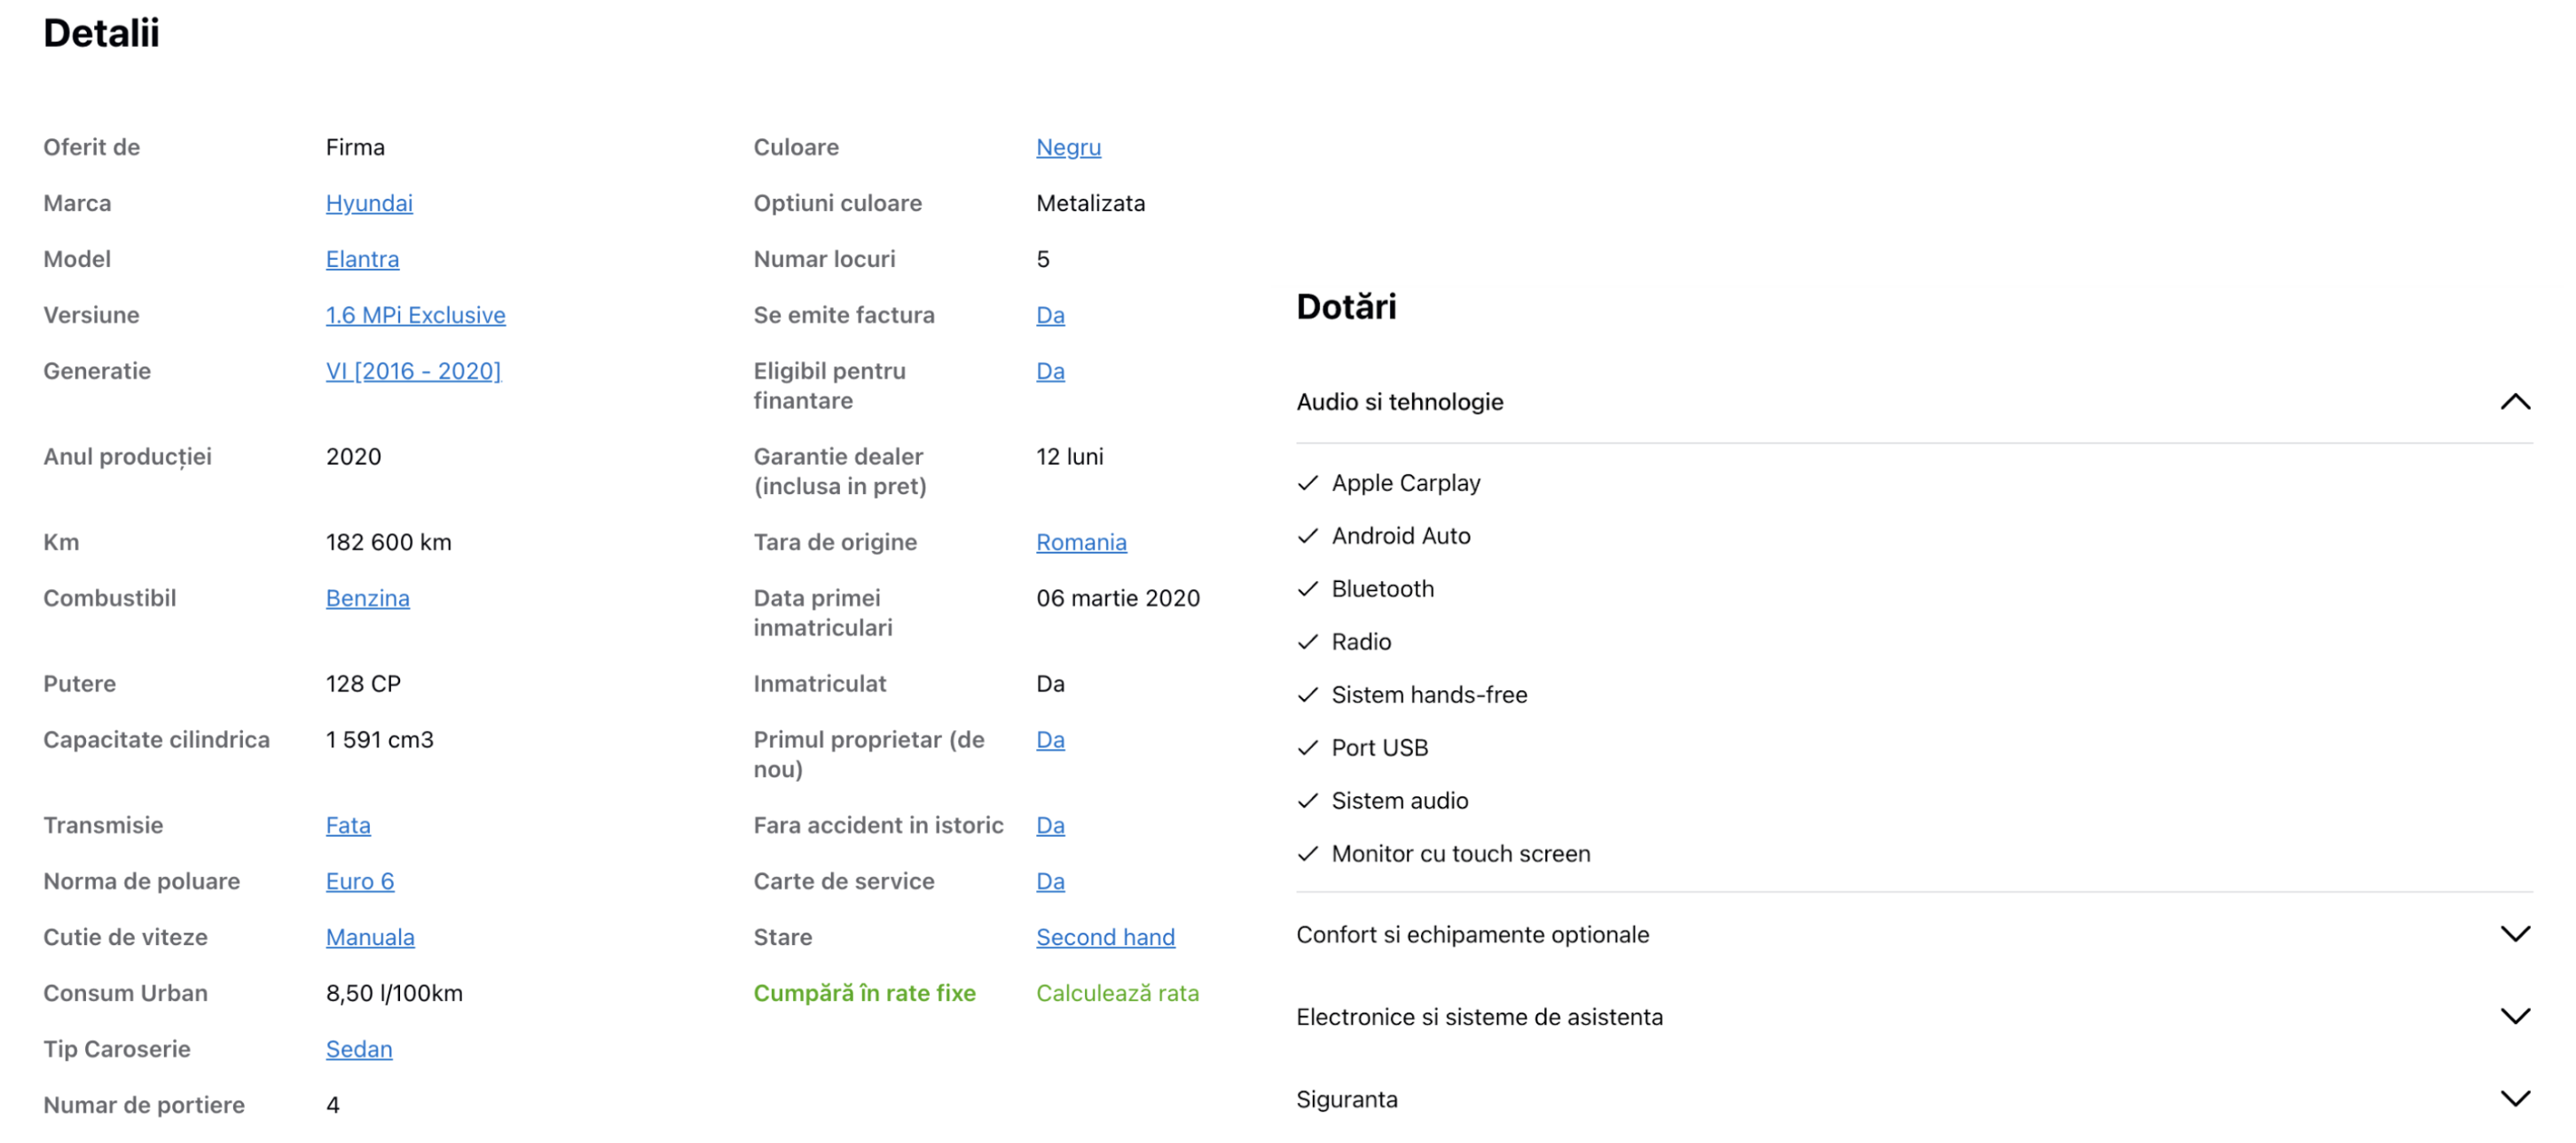
\includegraphics[width=\linewidth]{images/priceprediction/data/Screenshot 2024-05-28 at 21.33.53.png}
    \end{subfigure}
    \hfill
    \begin{subfigure}{\linewidth}
        \centering
        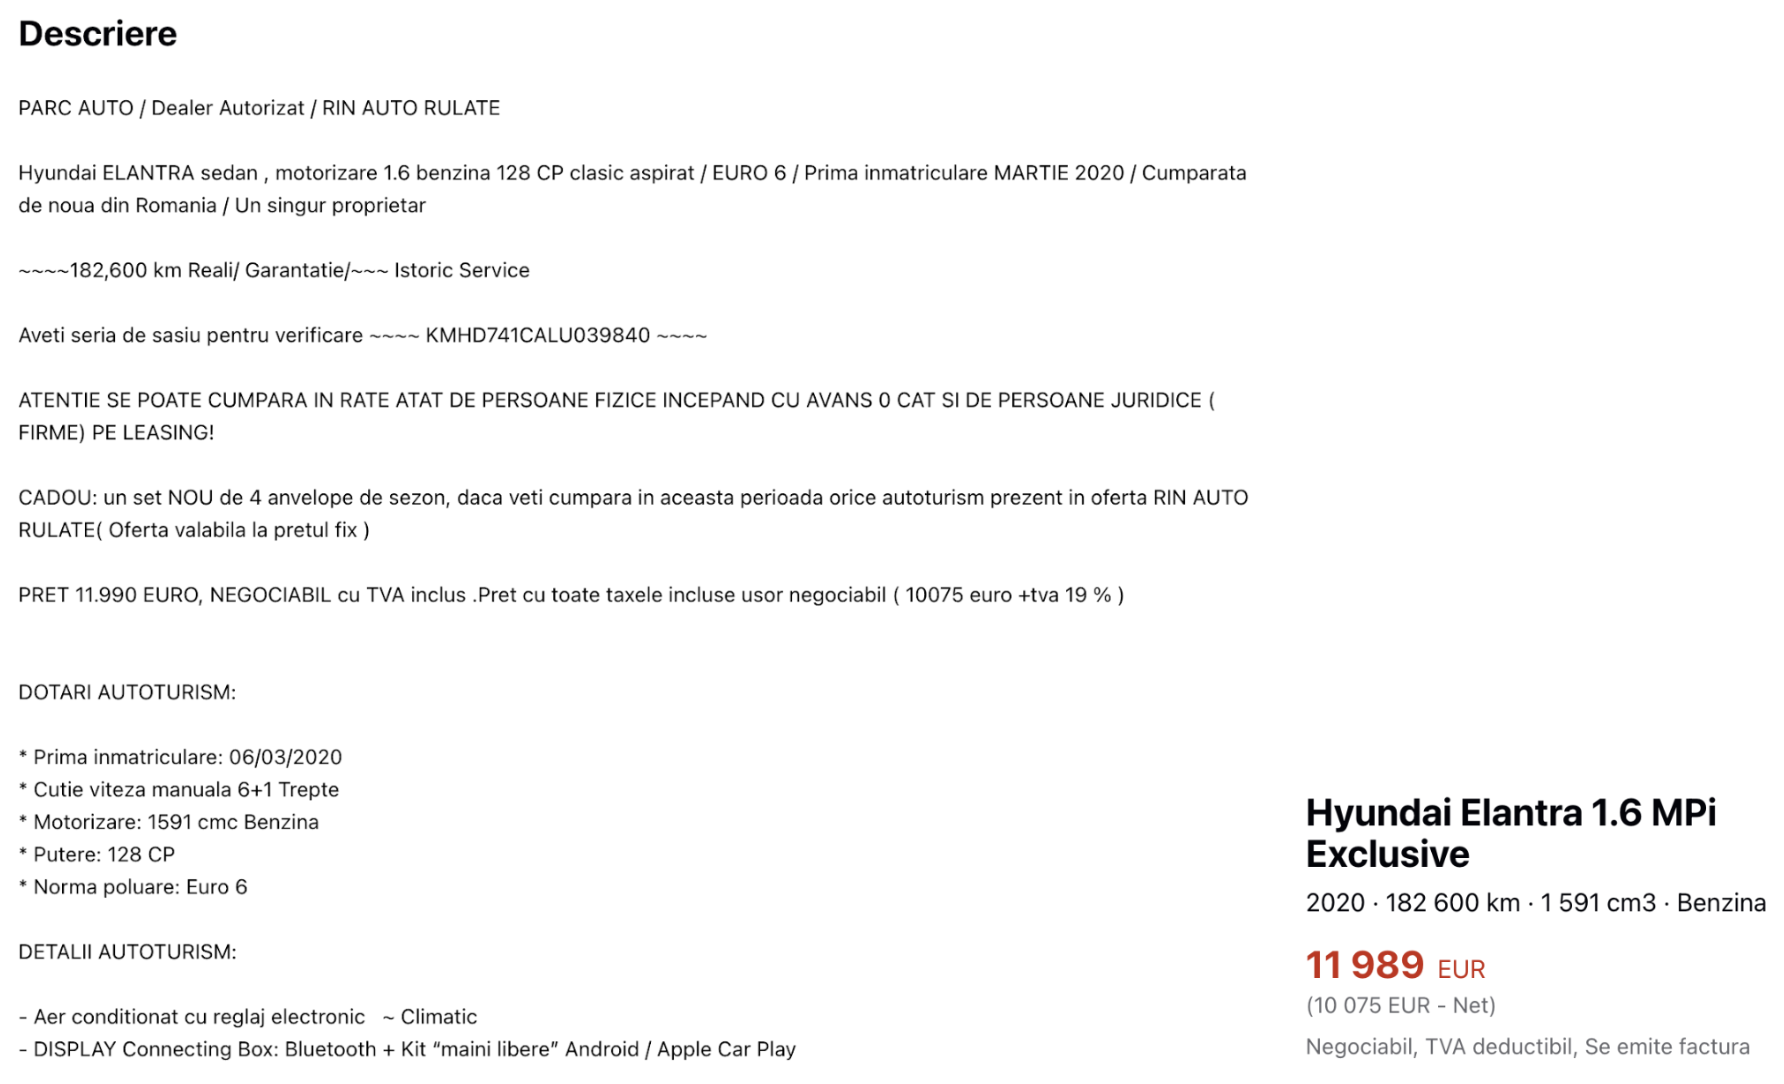
\includegraphics[width=\linewidth]{images/priceprediction/data/Screenshot 2024-05-28 at 21.39.39.png}
    \end{subfigure}
    \caption{Scraping Details}
    \label{fig:scraping-details}
\end{figure}

These stages formed a robust framework for our web scraping operations, ensuring efficient data collection and ongoing updates to support our machine learning model for car price prediction.

\subsection{Challenges and Solutions}
During the development and operation of our web scraping system, we encountered several challenges that required attention to ensure the effectiveness and efficiency of our data collection process. Here are the key challenges and the strategies we implemented to overcome them:

\begin{itemize}
    \item \textbf{Processing Speed}: Initially, the data scraping process was slow, hindering our ability to gather data efficiently. To address this, we implemented a multithreaded approach. This allowed us to execute multiple scraping operations in parallel, significantly reducing the time required to navigate through and download data from web pages. The enhancement in speed enabled us to handle larger volumes of data within shorter time frames, making our data collection process much more efficient.

\begin{lstlisting}
with ThreadPoolExecutor() as executor:
    futures = []

    for index, row in df.iterrows():
        future = executor.submit(process_row, df, index, row)
        futures.append(future)

    for future in futures:
        future.result()
\end{lstlisting}

    \item \textbf{Network Errors}: We frequently encountered network errors and timeouts, which disrupted the scraping process. To mitigate this, we implemented an automatic retry mechanism. Each failed request was automatically retried up to five times before the system moved on to the next task. This approach significantly reduced data loss due to transient network issues and ensured a higher success rate in data retrieval.

    \item \textbf{Limited Data Availability}: The Autovit platform restricts access to only the last 500 pages of listings, containing around 15,000 advertisements, which was insufficient for building a robust dataset. To overcome this limitation, we developed a recurring scraping strategy. By running our scraper weekly, we were able to continuously capture new listings as they were posted, adding approximately 5,000 new advertisements to our dataset each week. 
\end{itemize}

These solutions significantly improved our dataset, enabling us to construct a larger and more up-to-date dataset that effectively supports our car price prediction model.

\subsection{Ethical and Legal Considerations}
We ensured compliance with web scraping legal standards and Autovit’s terms of service \cite{AutovitTerms}, particularly regarding data privacy and usage policies.

\paragraph{The structure of our dataset after scraping is presented in \hyperref[tab:scraped-table]{Table 3.1}.}

\begin{longtable}{llll}
    \textbf{Category} & \textbf{No.} & \textbf{Features} & \textbf{D/C} \\ \hline
    \endfirsthead
    \multicolumn{4}{c}%
    {{\bfseries \tablename\ \thetable{} -- continued from previous page}} \\
    \hline
    \textbf{Category} & \textbf{No.} & \textbf{Features} & \textbf{D/C} \\ \hline
    \endhead
    \hline \multicolumn{3}{r}{{Continued on next page}} \\ \hline
    \endfoot
    \hline
    \endlastfoot

    \multirow{6}{*}{Custom options} & \multirow{6}{*}{6} & audio \& technology & continuous \\ 
    & & comfort \& optional equipment & continuous \\ 
    & & electronics \& assistance systems & continuous \\ 
    & & performance & continuous \\ 
    & & safety & continuous \\ 
    & & electric vehicles & continuous \\ \hline
    
    \multirow{23}{*}{General} & \multirow{23}{*}{23} & manufacturer & discrete \\ 
    & & model & discrete \\ 
    & & version & discrete \\ 
    & & year & continuous \\ 
    & & km & continuous \\ 
    & & sold by & discrete \\ 
    & & has vin (chassis number) & discrete \\ 
    & & fuel & discrete \\ 
    & & power & continuous \\ 
    & & engine capacity & continuous \\ 
    & & gearbox & discrete \\ 
    & & chassis & discrete \\ 
    & & doors & continuous \\ 
    & & color & discrete \\ 
    & & color options & discrete \\ 
    & & seats & continuous \\ 
    & & description & continuous \\ 
    & & price & continuous \\ 
    & & currency & discrete \\ 
    & & generation & continuous \\ 
    & & vintage car & discrete \\ 
    & & tuning & discrete \\ 
    & & right hand drive & discrete \\ \hline
    
    \multirow{5}{*}{Electric Vehicles Related} & \multirow{5}{*}{5} & range & continuous \\ 
    & & battery capacity & continuous \\ 
    & & manufacturer warranty until & continuous \\ 
    & & battery contract & continuous \\ 
    & & charging time & continuous \\ \hline
    
    \multirow{4}{*}{Fuel Consumption Related} & \multirow{4}{*}{4} & extra-urban consumption & continuous \\ 
    & & urban consumption & continuous \\ 
    & & combined consumption & continuous \\ 
    & & average consumption & continuous \\ \hline
    
    \multirow{2}{*}{Pollution Related} & \multirow{2}{*}{2} & co2 emissions & continuous \\ 
    & & pollution norm & discrete \\ \hline
    
    \multirow{8}{*}{Leasing Related} & \multirow{8}{*}{8} & invoice issued & discrete \\ 
    & & eligible for financing & discrete \\ 
    & & dealer warranty (included in price) & discrete \\ 
    & & leasing transfer & discrete \\ 
    & & initial payment (on delivery) & continuous \\ 
    & & monthly payment amount & continuous \\ 
    & & number of monthly payments remaining & continuous \\ 
    & & residual value & continuous \\ \hline
    
    \multirow{7}{*}{History Related} & \multirow{7}{*}{7} & country of origin & discrete \\ 
    & & first registration date & continuous \\ 
    & & registered & discrete \\ 
    & & first owner & discrete \\ 
    & & undamaged history & discrete \\ 
    & & service book & discrete \\ 
    & & condition & discrete \\ \hline
    \caption{Initial Scraped Dataset Structure}
    \label{tab:scraped-table}
\end{longtable}

\section{Data Formatting}

To ensure the accuracy and reliability of our predictive model, it was essential to standardize the raw data that we have scraped. The raw data contained numerous inconsistencies and mixed formats, which needed to be addressed through data formatting techniques.

The raw data presented several challenges:
\begin{itemize}
    \item \textbf{Numeric Data with Units}: Many numerical values were accompanied by units, making them unsuitable for direct use. For example, distances were recorded as "1237 km" instead of 1237.
    \item \textbf{Mixed Formats}: Other fields, such as the price, were in various formats. For example, some prices were listed as '1298.23', others as '1294,41', and some simply as 1239.
    \item \textbf{Romanian Booleans}: Boolean fields were scraped in Romanian as \textit{"da"} and \textit{"nu"}, which translate to \textit{True} and \textit{False}.
\end{itemize}

To address these issues, we employed various data formatting techniques:
\begin{itemize}
    \item \textbf{Removing Units from Numeric Data}: We used regular expressions in Python to strip units from numerical values. For instance, "1237 km" was converted to 1237.
    \item \textbf{Standardizing Measurement Units}: All measurements were standardized to ensure uniformity. For example, all prices were carefully converted to integers.
    \item \textbf{Converting Boolean Fields}: Boolean values were mapped from Romanian to English equivalents using a dictionary, converting \textit{"da"} to \textit{True} and \textit{"nu"} to \textit{False}.
\end{itemize}

\subsubsection{Enriching our descriptions}
In Romania's second-hand car market, it is common for sellers to highlight custom options and equipment in the description of their advertisements. This thing can be seen also in our example provided in \hyperref[fig:scraping-details]{Figure 3.1}. However, our data analysis revealed that some descriptions were either empty or lacked this specific information. 

To provide a more robust input to our BERT model, we appended our custom options columns \textit{audio \& technology, comfort \& optional equipment, electronics \& assistance systems, performance and safety} to the descriptions. We formatted these additions to match the enumerated style observed in most advertisements. By enriching the descriptions this way, we created a more consistent and comprehensive dataset, better aligned with the data we expect to encounter during future inference. Additionally, this step will be replicated by our inference endpoint if users provide more details on the custom options, which are unrequired fields.

A small example is the description in \hyperref[lst:description-before]{Listing 3.1} that will be concatenated with the text in \hyperref[lst:description-after]{Listing 3.2} after our enrichment process.

\begin{lstlisting}[caption={Raw Description}, label={lst:description-before}, language={}]
skoda octavia, 2.0 tdi, 140 cp, inmatriculata ro. eu*4.
in prezent la bord sunt 222.000 km. km 100% originali, toate documentele disponibile, carte service,
masina tinuta in garaj, caroseria fara accident, fara rugina, vopsea originala.
\end{lstlisting}

\begin{lstlisting}[caption={Custom Options for concatenation}, label={lst:description-after}, language={}]
audio si tehnologie: android auto,port usb,monitor cu touch screen,control vocal
confort si echipamente optionale: climatronic,incalzire scaun sofer,scaune sport,keyless entry
electronice si sisteme de asistenta: pilot automat,lane assist,controlul distantei,controlul tractiunii,sistem recunoastere semne trafic,asistenta faza lunga
siguranta: abs,esp,sistem avertizare pre-coliziune,isofix
\end{lstlisting}

\section{Data Cleaning}
\label{sec:data-cleaning}

Although our dataset is rich in features and samples, an initial analysis revealed many null values as shown in \hyperref[fig:scraped-null]{Figure 3.2}. Manually labeling the data was not feasible due to both time constraints and a lack of expertise in the automotive sector.

\begin{figure}[ht]
\centering
\label{fig:scraped-null}
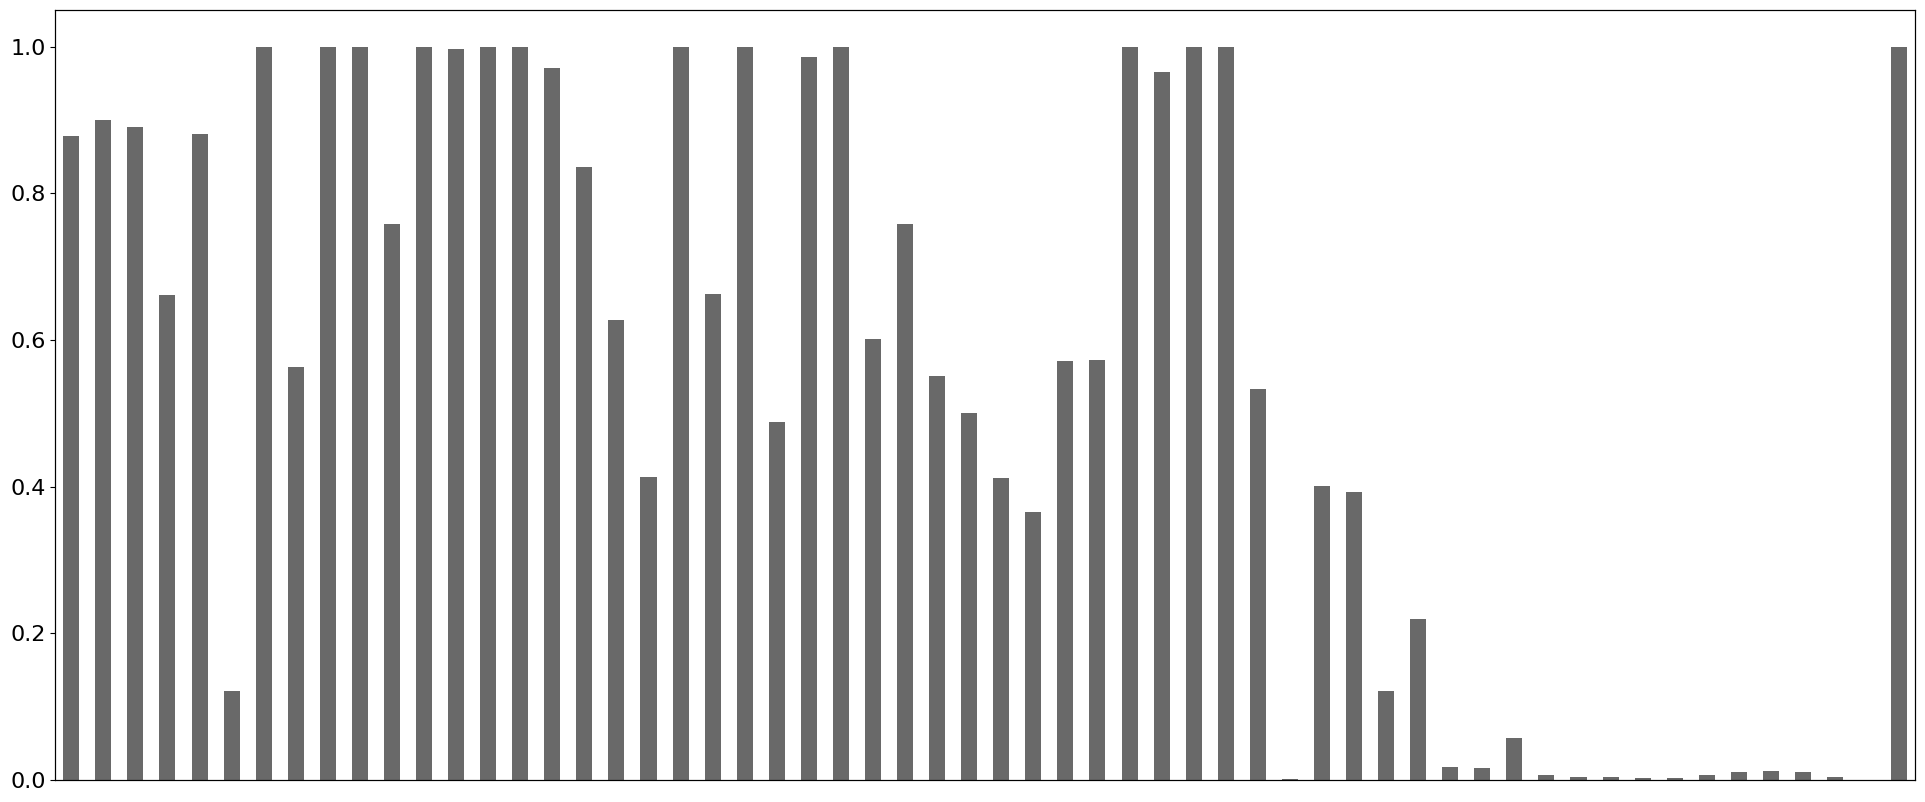
\includegraphics[width=1\linewidth]{priceprediction/data/null.png}
\caption{Histogram of non-null values in the scraped dataset across our features}
\end{figure}

Given this, we undertook an extensive removal process.

Effective data cleaning is crucial for ensuring the reliability and accuracy of our predictive model. The raw dataset contained several inconsistencies and irrelevant data points, which necessitated a thorough cleaning process. This section details the steps taken to clean the data, including the identification and removal of outliers, standardization of formats and types, and handling of missing values.

\subsection{Identifying and Removing Outliers}
\begin{enumerate}
    \item \textbf{Electric Vehicles}: Due to their really low number of appearances (1326) in our dataset, and also their specific price points, such as range, and battery capacity, we had to remove them completely.
    \item \textbf{Leasing Vehicles}: Vehicles listed under leasing agreements were also classified as outliers, being present in only 322 samples of such examples. The incomplete information on leasing terms and the difficulty in approximating their real prices led to their removal along with their specific columns.
    \item \textbf{Tuning}: Tuned cars were removed as they were considered outliers and lacked detailed information, which could vary significantly. We had only 482 such vehicles in our dataset.
\end{enumerate}

\subsection{Standardizing Data Formats}
\begin{itemize}
    \item \textbf{Price Data}: We decided to keep only prices that represent the EUR currency. Although the approach to convert the RON ones to their EUR equivalent seemed like the right decision at first glance, we detected some bad placed advertisement, that had their currency set to RON, but the price represented their actual EUR price. We remove 46 samples in total at this step.
    \item \textbf{Removing Error Prone Columns}: Columns with boolean values such as \textit{has vin (chassis number), vintage car, tuning, right-hand drive} where null values could not be assumed as False were removed to avoid introducing false negatives. 210 samples were removed.
\end{itemize}

\subsection{Handling Missing Values}
\begin{itemize}
    \item \textbf{Dropping Columns with High Null Values}: Due to a high number of null values, the following categories of columns were dropped: fuel consumption related, pollution related, and history related.
    \item \textbf{Selective Column Removal}: Certain columns from the general category, such as \textit{generation} and \textit{version}, were also removed due to their extremely sparse nature and high null appearances.
\end{itemize}

\subsection{Removing structured data outliers}
Although we previously removed several outliers from our dataset, such as electric vehicles and tuned cars, resulting in a more robust and complete dataset presented in \hyperref[tab:cleaned-table]{Table 3.2}, further analysis revealed that multiple key parameters still contained outliers. These outliers, if left unaddressed, could skew the results of our predictive model.

During our initial phases of data analysis, we identified several key metrics with significant outliers in terms of the number of samples. To ensure the robustness and accuracy of our model, we applied additional filtering criteria to remove these outliers, while still maintaining a good range of generalization.

\textbf{Power}: We filtered out vehicles with power greater than 600 HP or less than 50 HP. These values were deemed unrealistic for most vehicles in our dataset and would have introduced unnecessary noise into our model.

\begin{lstlisting}
df = df[df["power"] <= 600]
df = df[df["power"] >= 50]
# power: removed 218 rows
\end{lstlisting}

\textbf{Engine Capacity}: Vehicles with an engine capacity less than 500 cc or greater than 4000 cc were removed. This range was selected to exclude some badly placed advertisements, such as motorcycles, trucks, and other vehicles not representative of standard passenger cars.

\begin{lstlisting}
df = df[df["engine capacity"] >= 500]
df = df[df["engine capacity"] <= 4000]
# engine capacity: removed 305 rows
\end{lstlisting}

\textbf{Price}: We excluded vehicles with prices exceeding 40,000 EUR. These high-priced cars constituted a very small subset of our dataset and often included luxury or rare models that do not reflect general market trends. Additionally, buyers interested in such expensive cars typically rely on professional businesses for evaluation, making them outside the scope of our target market.

\begin{lstlisting}
df = df[df["price"] <= 40_000]
# price: removed 3911 rows
\end{lstlisting}

\textbf{Kilometers Driven}: Cars with more than 500,000 kilometers were removed, as they were also a small subset in our dataset.

\begin{lstlisting}
df = df[df["km"] <= 500_000]
# km: removed 30 rows
\end{lstlisting}

\textbf{Manufacturer Count}: We filtered out manufacturers with fewer than 100 listings in the dataset. Since the manufacturer and model are crucial factors in price prediction, brands with limited listings could skew the results due to insufficient data. By focusing on more common manufacturers, we create a more balanced and reliable dataset.

\begin{lstlisting}
temp_df = df["manufacturer"].value_counts()
df = df[df["manufacturer"].isin(temp_df[temp_df >= 100].index)]
# manufacturer: removed 482 rows
\end{lstlisting}

All these outliers are visually illustrated in \hyperref[fig:outliers]{Figure 3.3}.

\begin{figure}[ht]
    \centering
    \begin{subfigure}[b]{0.32\linewidth}
        \centering
        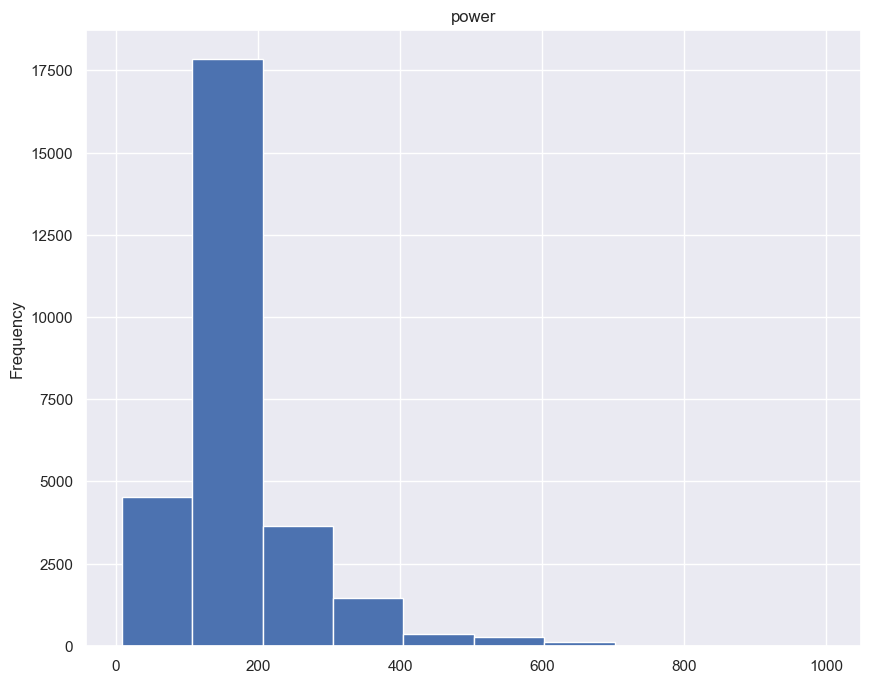
\includegraphics[width=\linewidth]{images/priceprediction/outliers/power.png}
        \caption{power}
        \label{fig:power}
    \end{subfigure}
    \hfill
    \begin{subfigure}[b]{0.32\linewidth}
        \centering
        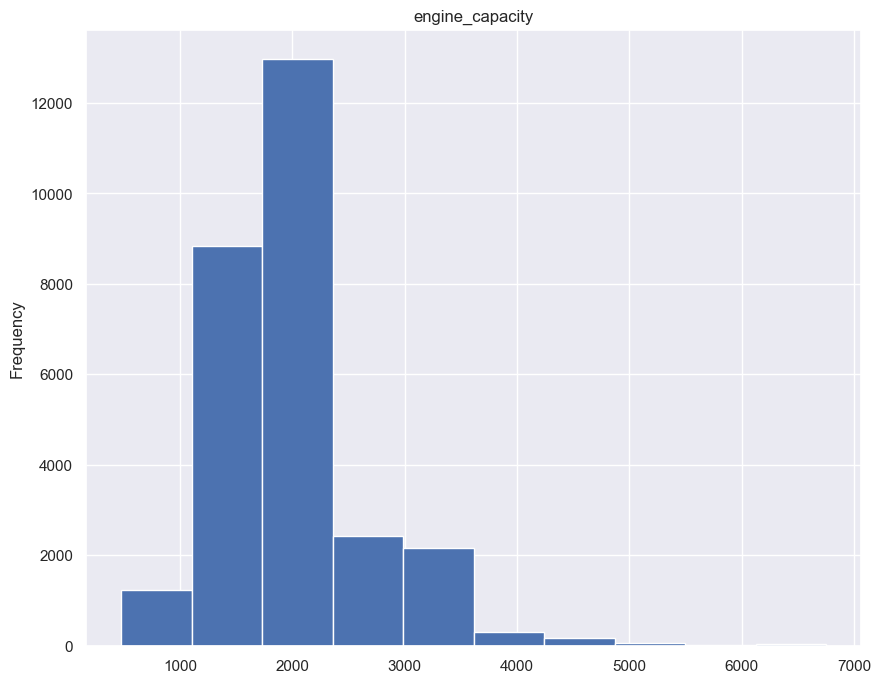
\includegraphics[width=\linewidth]{images/priceprediction/outliers/engine_capacity.png}
        \caption{engine\_capacity}
        \label{fig:engine_capacity}
    \end{subfigure}
    \hfill
    \begin{subfigure}[b]{0.32\linewidth}
        \centering
        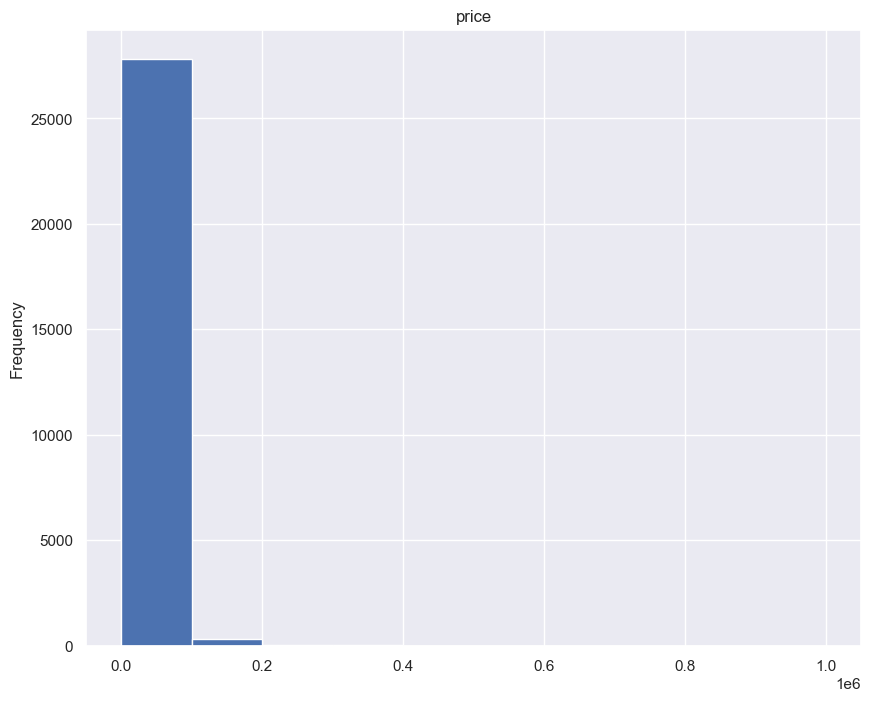
\includegraphics[width=\linewidth]{images/priceprediction/outliers/price.png}
        \caption{price}
        \label{fig:price}
    \end{subfigure}
    \vfill
    \begin{subfigure}[b]{0.48\linewidth}
        \centering
        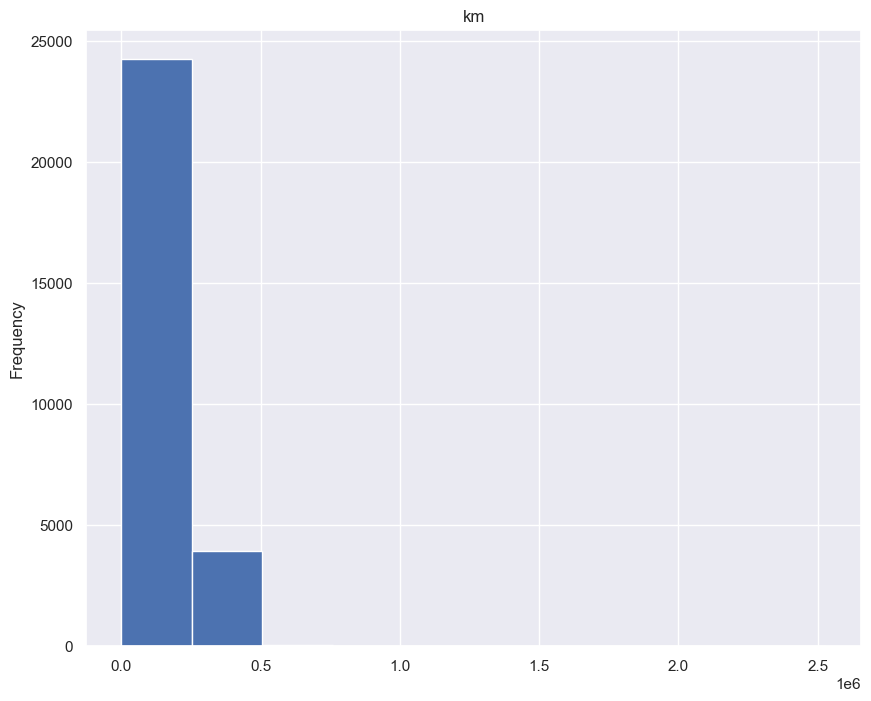
\includegraphics[width=\linewidth]{images/priceprediction/outliers/km.png}
        \caption{km}
        \label{fig:km}
    \end{subfigure}
    \hfill
    \begin{subfigure}[b]{0.48\linewidth}
        \centering
        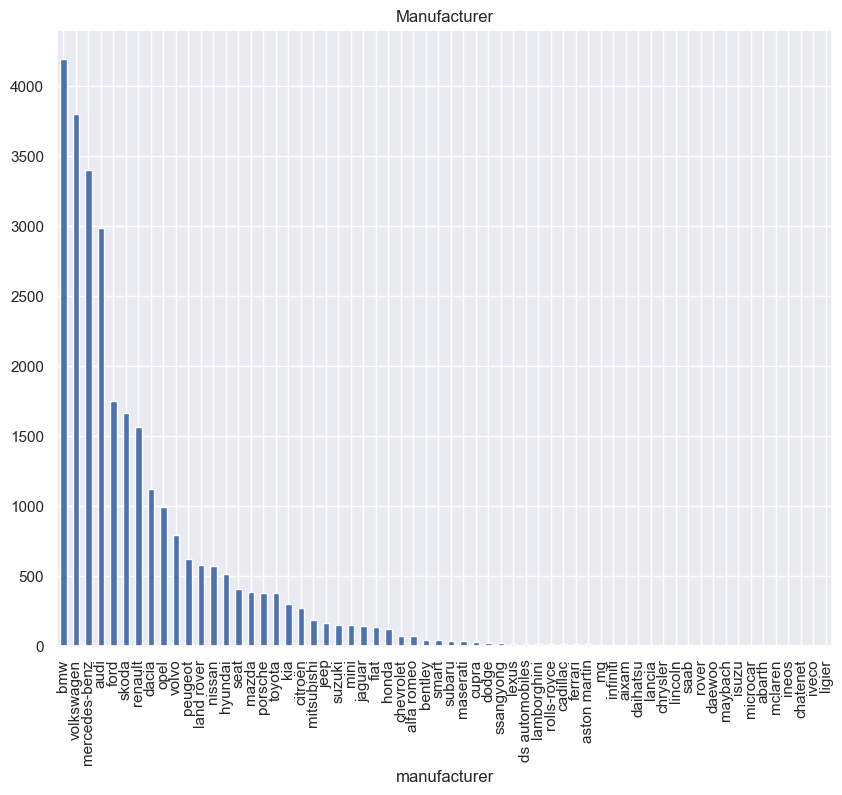
\includegraphics[width=\linewidth]{images/priceprediction/outliers/manufacturer.png}
        \caption{manufacturer\_count}
        \label{fig:manufacturer_count}
    \end{subfigure}
    \caption{Histograms of various features before filtering}
    \label{fig:outliers}
\end{figure}


\paragraph{The final structure of our dataset is presented in \hyperref[tab:cleaned-table]{Table 3.2}.}

\begin{longtable}{llll}
    \textbf{Column} & \textbf{Discrete/Continuous} & \textbf{Type} \\ \hline
    price & continuous & number \\ \hline
    manufacturer & discrete & text  \\ \hline
    model & discrete  & text \\ \hline
    year & continuous & number \\ \hline
    km & continuous & number \\ \hline
    power & continuous  & number \\ \hline
    engine capacity & continuous & number \\ \hline
    fuel & discrete & text \\ \hline
    chassis & discrete & text \\ \hline
    is\_automatic & discrete & boolean \\ \hline
    sold\_by\_company & discrete & boolean \\ \hline
    description & continuous & text \\ \hline
    \caption{Final Dataset Structure}
    \label{tab:cleaned-table}
\end{longtable}


\section{Data Analysis}
This section is divided into two subsections: structured data analysis and unstructured data analysis. Each subsection aims to provide a comprehensive understanding of the dataset by examining different types of data and extracting meaningful insights, while also validating our dataset.

\subsection{Structured Data}
In this subsubsection, we focus on analyzing the structured data, including both numerical and categorical variables. This analysis helps in understanding the distributions, relationships, and patterns within the dataset.

\subsubsection{Numerical Data Analysis}

\begin{itemize}
    \item \textbf{Price}: The histogram of car prices reveals a right-skewed distribution, with most cars priced between 5,000 and 15,000 EUR. This skewness indicates a higher concentration of lower-priced vehicles, which is typical for a second-hand car market.

    \begin{figure}[!h]
        \centering
        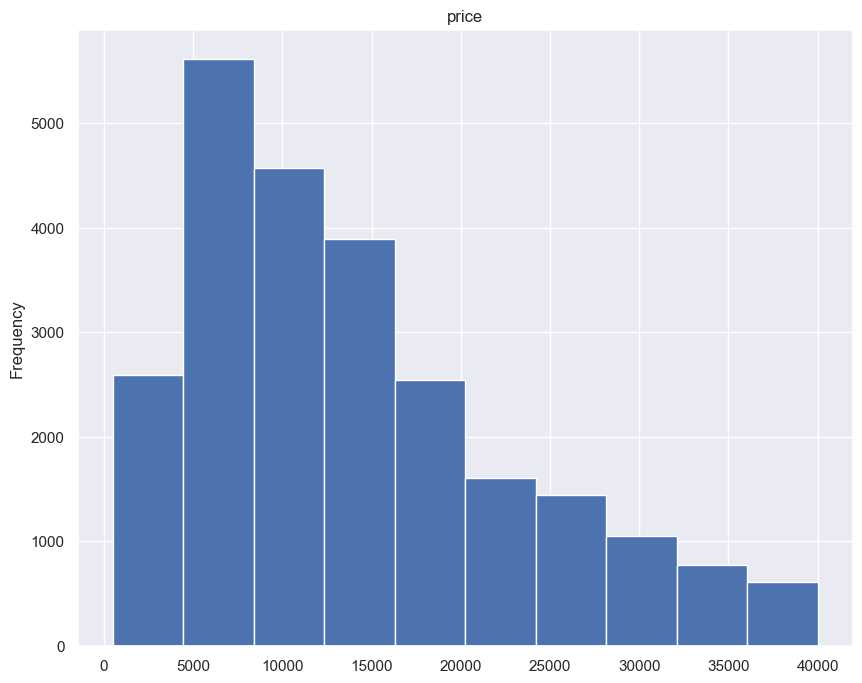
\includegraphics[width=0.5\linewidth]{images/priceprediction/after_outliers/price.png}
        \caption{Price Histogram}
        \label{fig:price-hist}
    \end{figure}

    \item \textbf{Year}: The year of manufacture is a critical factor in estimating a car's selling price. The histogram in \hyperref[fig:year-hist]{Figure 3.5 (a)} shows that most advertisements are for cars that are five to ten years old, with fewer listings for older vehicles. This reflects market trends favoring newer models. Additionally, the correlation between price and year of manufacture shown in \hyperref[fig:year-box]{Figure 3.5 (b)} aligns with real-world data, where newer cars typically command higher prices.
    
    \begin{figure}[ht]
        \begin{subfigure}[b]{0.48\linewidth}
            \centering
            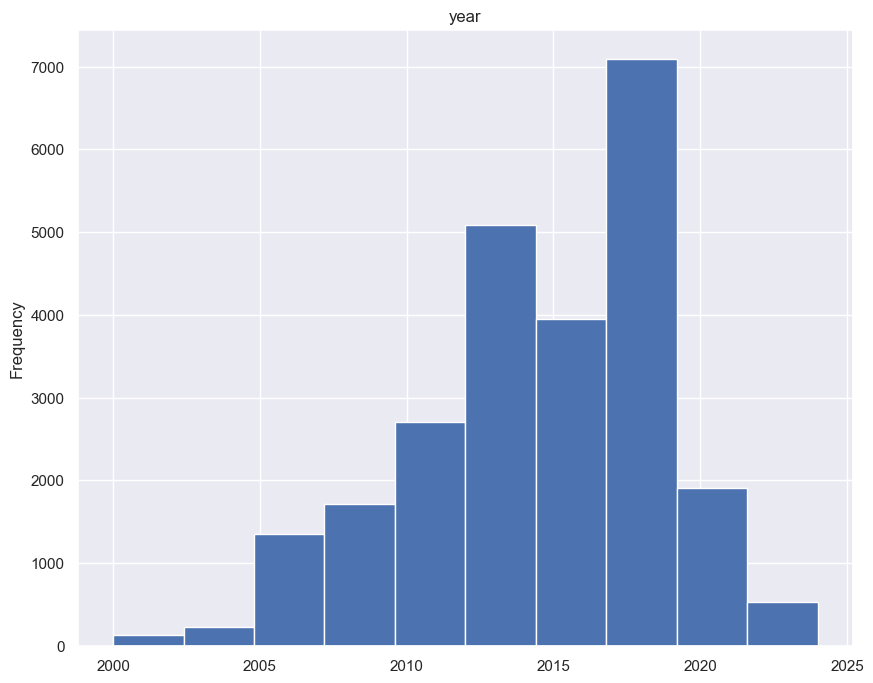
\includegraphics[width=\linewidth]{images/priceprediction/after_outliers/year.png}
            \caption{Year Histogram}
            \label{fig:year-hist}
        \end{subfigure}
        \hfill
        \begin{subfigure}[b]{0.48\linewidth}
            \centering
            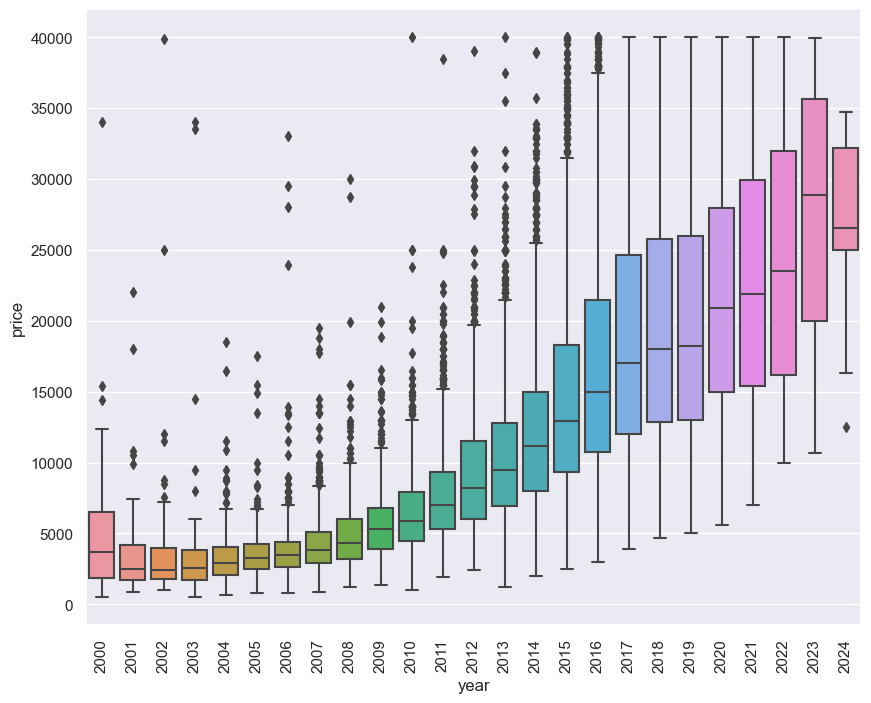
\includegraphics[width=\linewidth]{images/priceprediction/boxplots/year_price.png}
            \caption{Box plot price \& year}
            \label{fig:year-box}
        \end{subfigure}
        \caption{Year analysis}
        \label{fig:year}
    \end{figure}

     \item \textbf{Kilometers}: The distribution of kilometers driven, as shown in \hyperref[fig:km-hist]{Figure 3.6 (a)}, indicates that most cars have mileage between 100,000 and 250,000 kilometers. Higher mileage vehicles are less common, reflecting the typical lifespan of cars and their lower market value. This trend is observed in \hyperref[fig:km-box]{Figure 3.6 (b)}, where cars with higher mileage tend to be cheaper, aligning with the market preference for relatively low-mileage vehicles.

     \begin{figure}[!h]
        \begin{subfigure}[b]{0.48\linewidth}
            \centering
            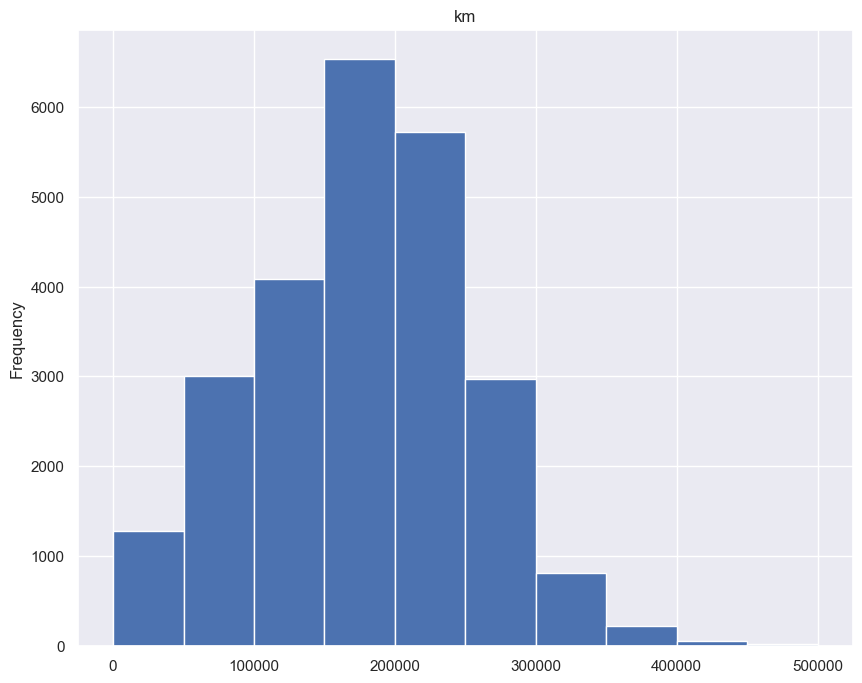
\includegraphics[width=\linewidth]{images/priceprediction/after_outliers/km.png}
            \caption{Kilometers Histogram}
            \label{fig:km-hist}
        \end{subfigure}
        \hfill
        \begin{subfigure}[b]{0.48\linewidth}
            \centering
            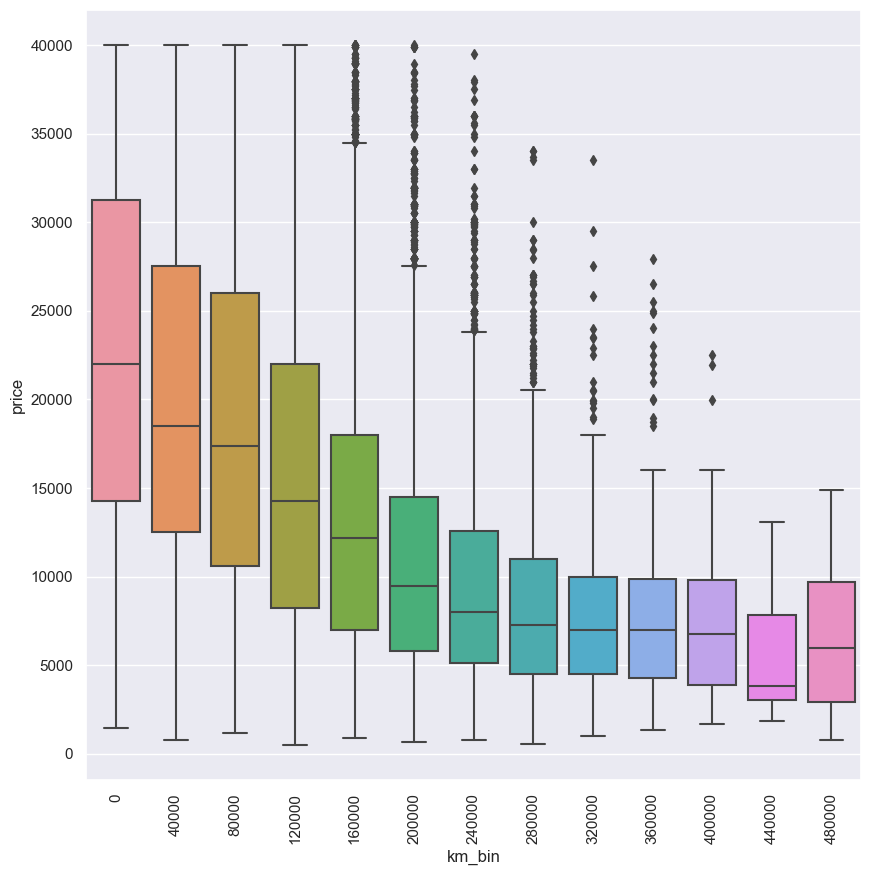
\includegraphics[width=\linewidth]{images/priceprediction/boxplots/km_price.png}
            \caption{Box plot price \& kilometers}
            \label{fig:km-box}
        \end{subfigure}
        \caption{Kilometers driven analysis}
        \label{fig:km}
    \end{figure}

    \item \textbf{Power and Engine Capacity}: Both power and engine capacity have a strong positive correlation with price. Higher power and larger engine capacity lead to higher selling prices due to their performance capabilities and appeal to buyers seeking more powerful vehicles, evidenced in \hyperref[fig:pow-eng-box]{Figure 3.7}.

    \begin{figure}[!h]
        \begin{subfigure}[b]{0.48\linewidth}
            \centering
            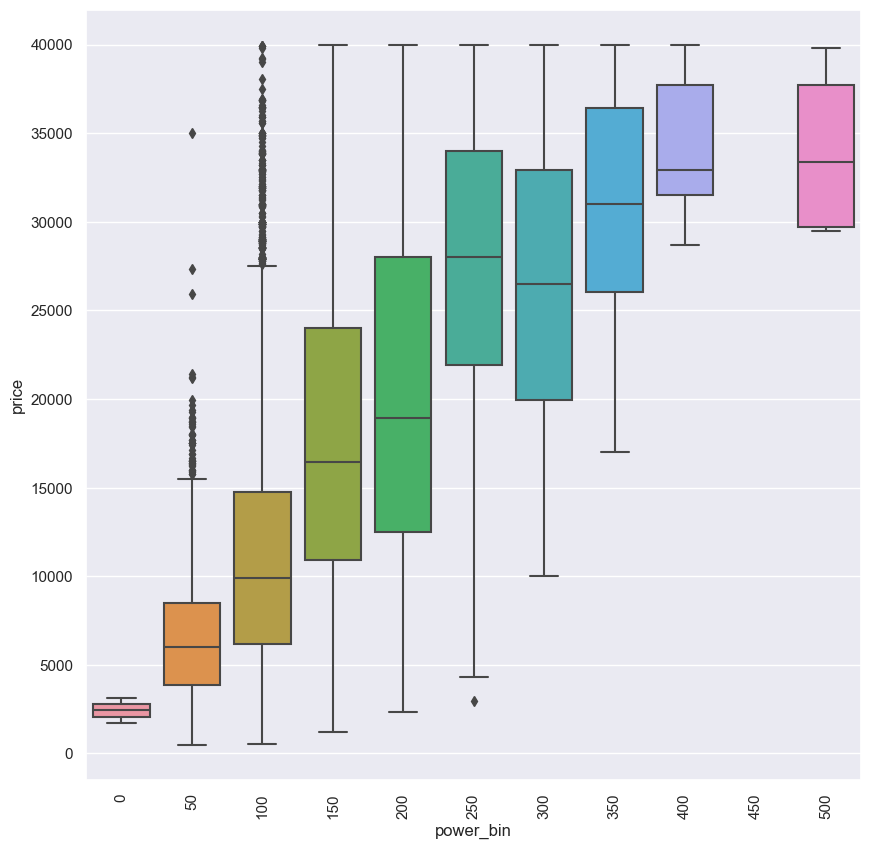
\includegraphics[width=\linewidth]{images/priceprediction/boxplots/power_price.png}
            \caption{Box plot price \& power}
            \label{fig:power-box}
        \end{subfigure}
        \hfill
        \begin{subfigure}[b]{0.48\linewidth}
            \centering
            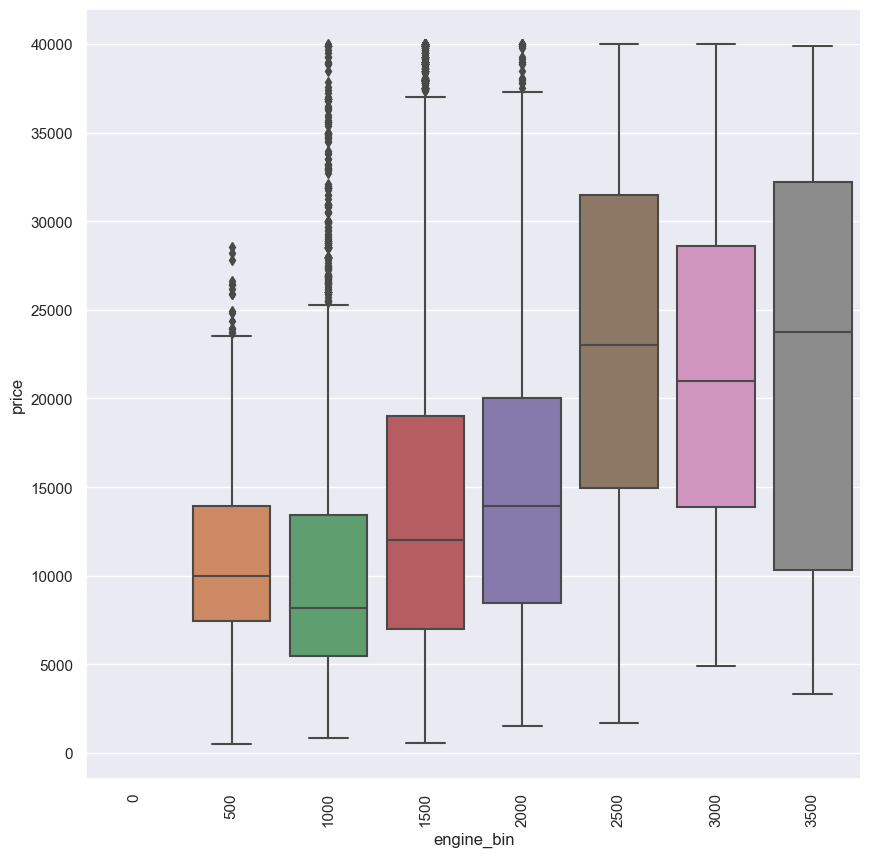
\includegraphics[width=\linewidth]{images/priceprediction/boxplots/engine_capacity_price.png}
            \caption{Box plot price \& engine\_capacity}
            \label{fig:eng-box}
        \end{subfigure}
        \caption{Power \& engine capacity analysis}
        \label{fig:pow-eng-box}
    \end{figure}
    
\end{itemize}

\subsubsection{Categorical Data Analysis}

\begin{itemize}
    \item \textbf{Manufacturer}: The bar chart in \hyperref[fig:manufacturer-hist]{Figure 3.8 (a)} illustrates the frequency of different car brands, with Volkswagen, BMW, and Audi being the most common. Additionally, the box plot in \hyperref[fig:manufacturer-box]{Figure 3.8 (b)} shows the relationship between manufacturers and prices, indicating that some brands, such as Mercedes, Porsche, and Volvo, tend to be pricier. This is expected, as these manufacturers primarily produce luxury vehicles, which command higher prices in the used cars market.

    \begin{figure}[!h]
        \begin{subfigure}[b]{0.48\linewidth}
            \centering
            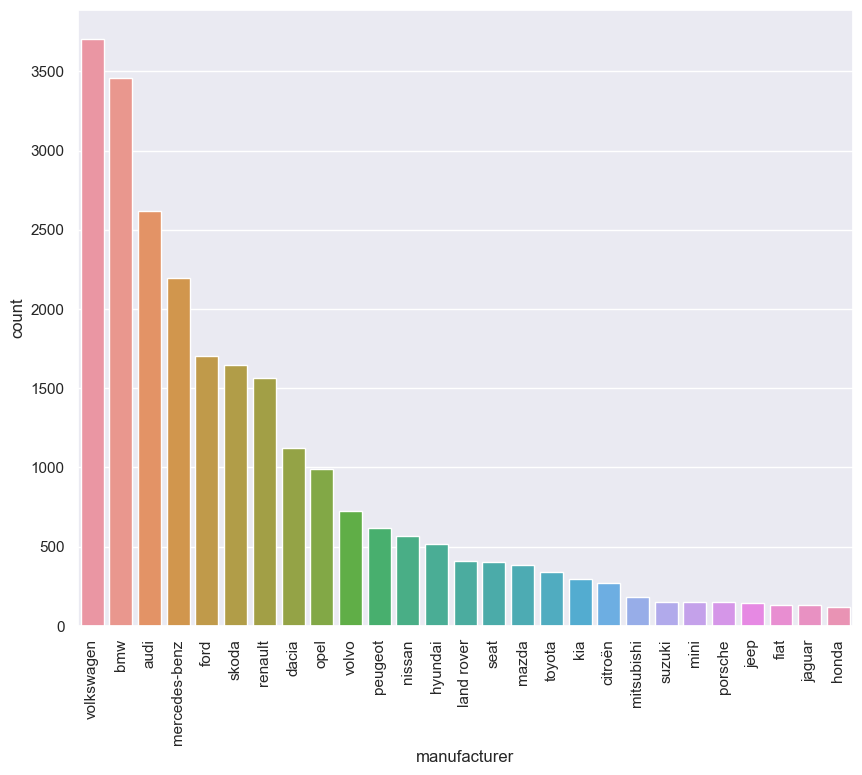
\includegraphics[width=\linewidth]{images/priceprediction/histograms/manufacturer-hist.png}
            \caption{Manufacturer Histogram}
            \label{fig:manufacturer-hist}
        \end{subfigure}
        \hfill
        \begin{subfigure}[b]{0.48\linewidth}
            \centering
            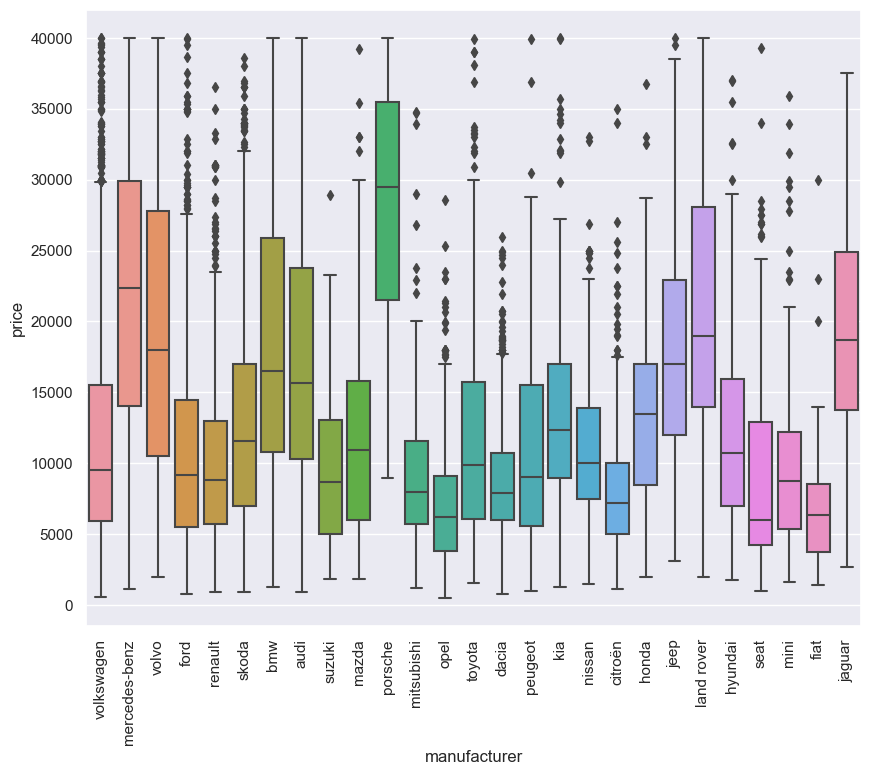
\includegraphics[width=\linewidth]{images/priceprediction/boxplots/manufacturer_price.png}
            \caption{Box plot price \& manufacturer}
            \label{fig:manufacturer-box}
        \end{subfigure}
        \caption{Manufacturer Analysis}
        \label{fig:manufacturer-analysis}
    \end{figure}
    
    \item \textbf{Fuel \& Chassis}: The correlation between fuel type and price, as well as chassis type and price, shown in \hyperref[fig:fuel-chassis-analysis]{Figure 3.9}, indicates that diesel cars are slightly more expensive, likely due to their renowned reliability. Additionally, coupes and SUVs tend to command higher prices compared to smaller city cars, owing to their more appealing and stately appearance.

    \begin{figure}[!h]
        \begin{subfigure}[b]{0.48\linewidth}
            \centering
            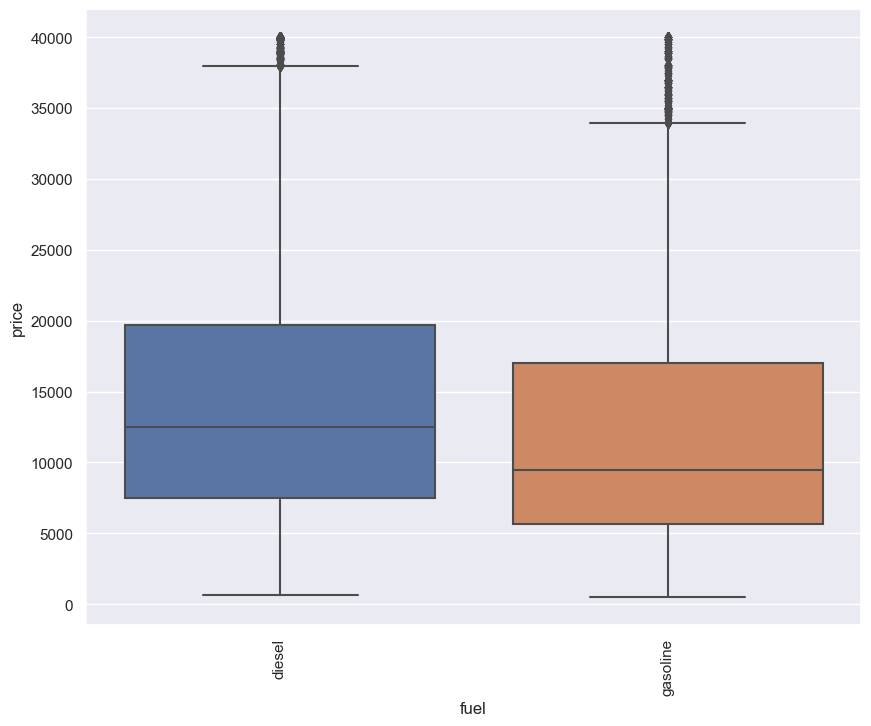
\includegraphics[width=\linewidth]{images/priceprediction/boxplots/fuel_price.png}
            \caption{Box plot price \& fuel}
            \label{fig:fuel-box}
        \end{subfigure}
        \hfill
        \begin{subfigure}[b]{0.48\linewidth}
            \centering
            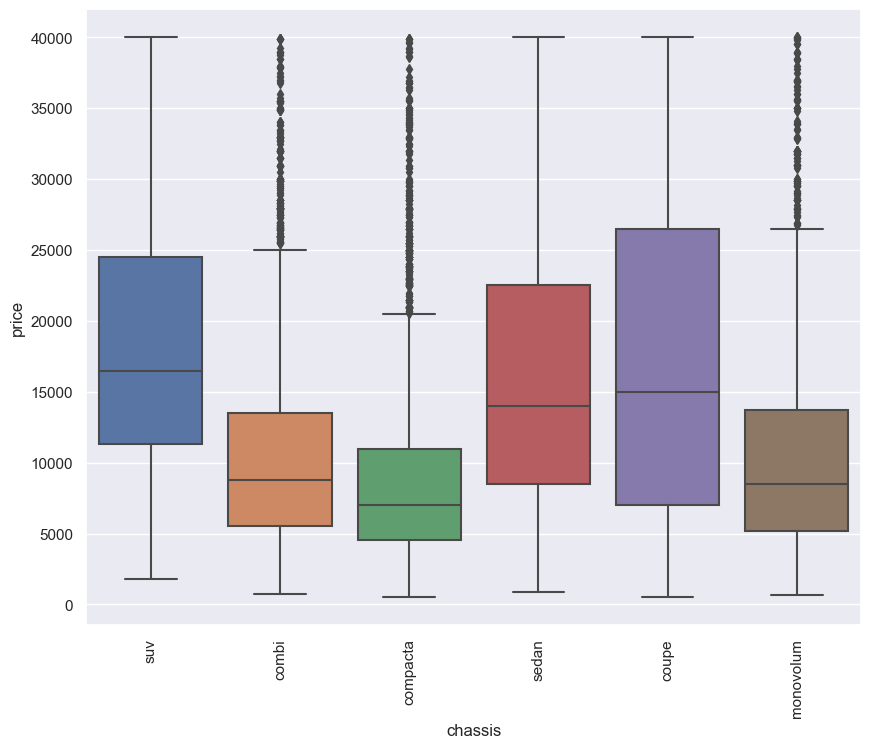
\includegraphics[width=\linewidth]{images/priceprediction/boxplots/chassis_price.png}
            \caption{Box plot price \& chassis}
            \label{fig:chassis-box}
        \end{subfigure}
        \caption{Fuel \& Chassis Analysis}
        \label{fig:fuel-chassis-analysis}
    \end{figure}

    \item \textbf{Gearbox \& Seller}: In \hyperref[fig:gearbox-seller-analysis]{Figure 3.10}, there is a clear relationship between gearbox type and price, with automatic cars fetching higher resale prices due to the comfort they provide. Furthermore, cars sold by businesses are generally priced higher, as these sellers include their profit margins in the resale price.

    \begin{figure}[!h]
        \begin{subfigure}[b]{0.48\linewidth}
            \centering
            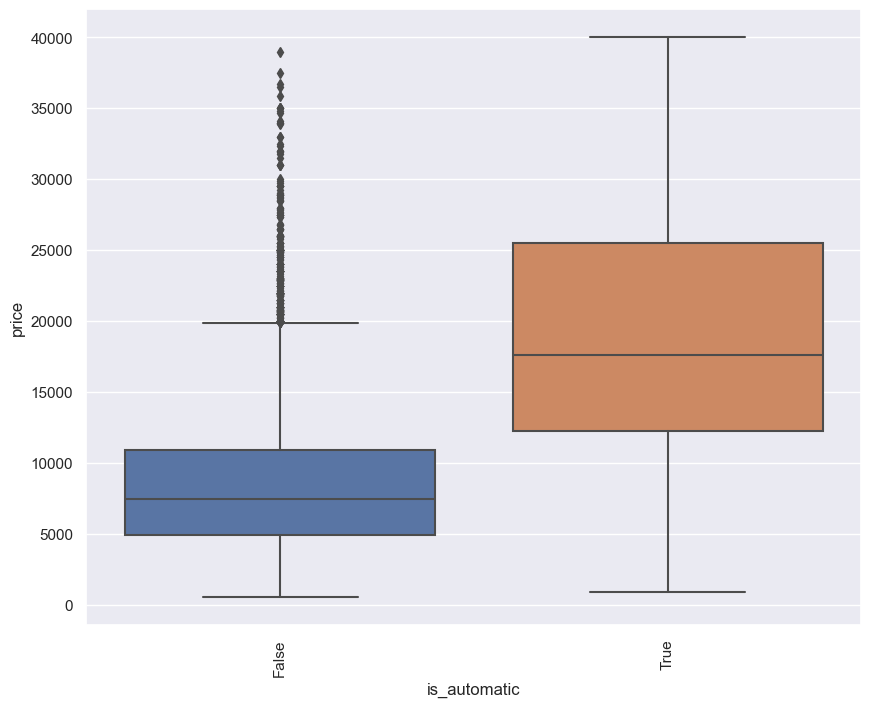
\includegraphics[width=\linewidth]{images/priceprediction/boxplots/is_automatic_price.png}
            \caption{Box plot price \& gerabox}
            \label{fig:gearbox-box}
        \end{subfigure}
        \hfill
        \begin{subfigure}[b]{0.48\linewidth}
            \centering
            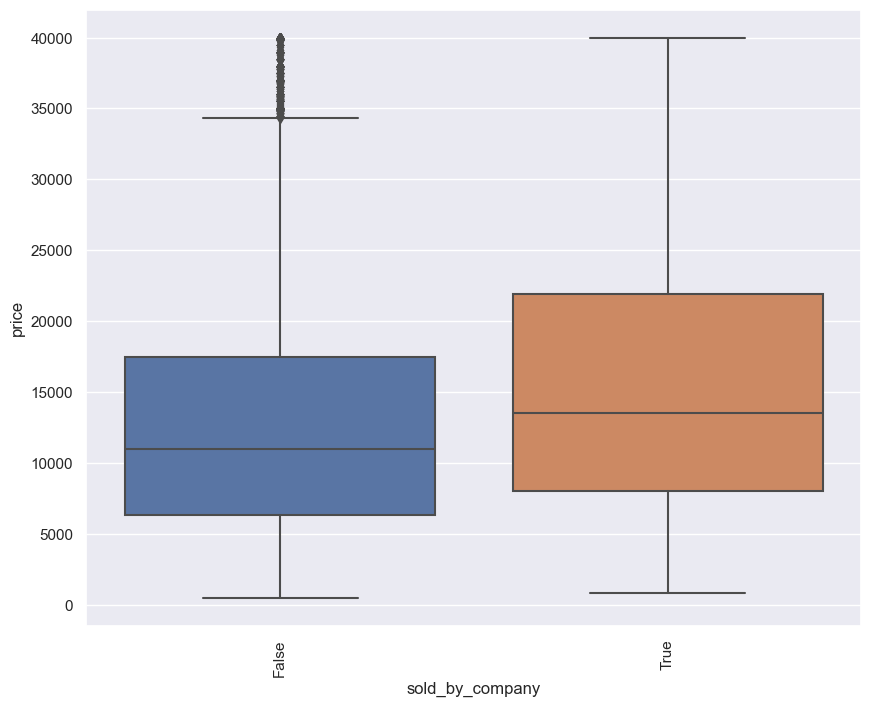
\includegraphics[width=\linewidth]{images/priceprediction/boxplots/sold_by_company_price.png}
            \caption{Box plot price \& seller}
            \label{fig:seller-box}
        \end{subfigure}
        \caption{Gearbox \& Seller Analysis}
        \label{fig:gearbox-seller-analysis}
    \end{figure}
    
\end{itemize}

\subsection{Unstructured Data}
This subsection focuses on the analysis of unstructured data, including text descriptions and images. These analyses complement the structured data insights and provide a more holistic understanding of the dataset.


\subsubsection{Image Data Analysis}

The analysis of images was conducted manually, primarily observing the following aspects:

\begin{itemize}
    \item In the images resulting from the scraping process, we failed to identify a pattern in the angles from which the photos were taken. While advertisements posted by companies tend to have more professional photos, as showcased in \hyperref[fig:sample-images]{Figure 3.11}, the ones posted by normal users have various formats. We've conducted manual selection, trying to select similar angles throughout our dataset by selecting front-to-side pictures for each sample. Luckily, our decision to scrape ten images for each entry gave us a big enough selection pool to achieve this.
    \item Some company-posted advertisements include banners, as seen in \hyperref[fig:sample-images]{Figure 3.11}, which could confuse our feature extraction model. This issue was also mitigated by manually selecting one image per sample without such banners.
\end{itemize}

\begin{figure}[ht]
    \centering
    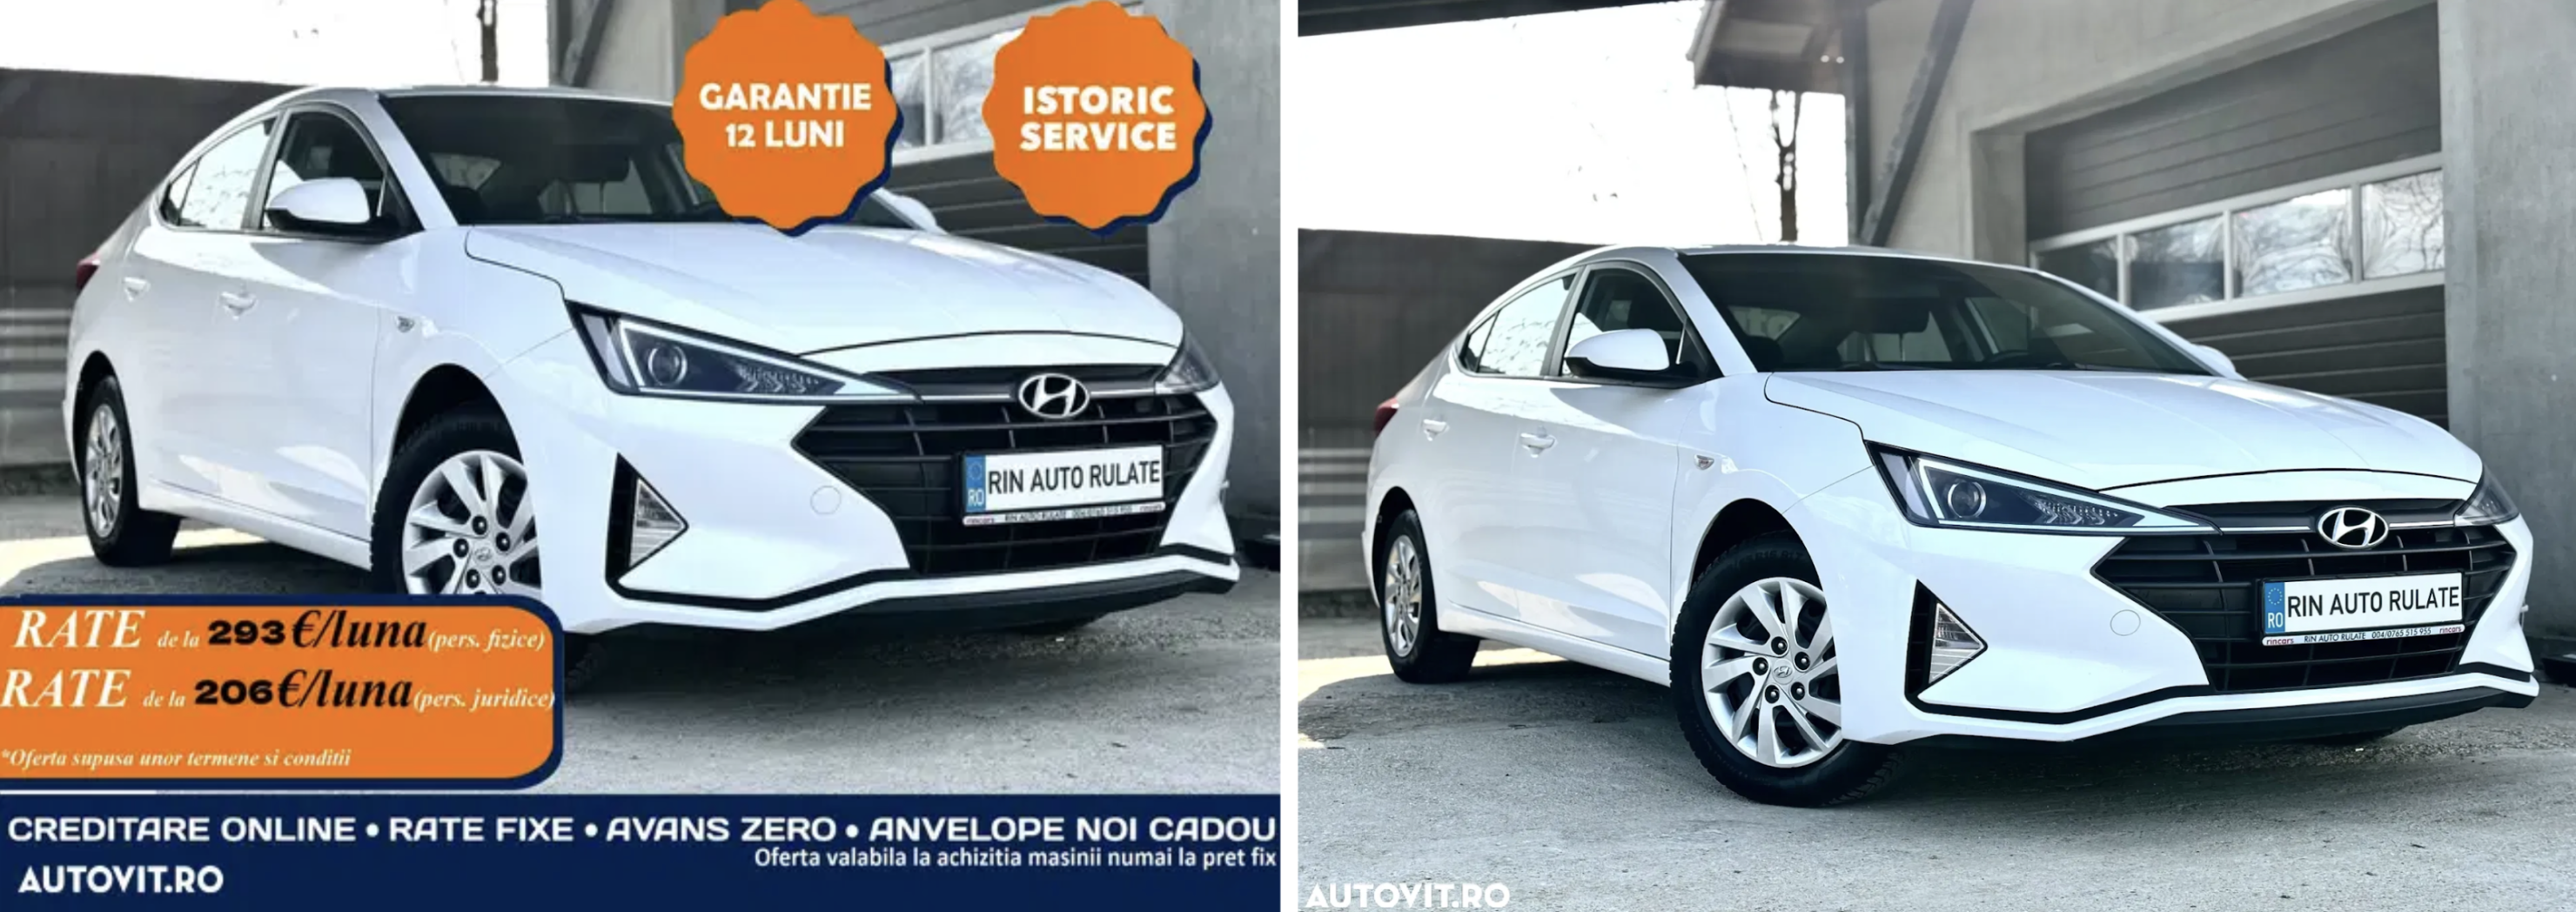
\includegraphics[width=1\linewidth]{images/priceprediction/data/Screenshot 2024-05-28 at 21.33.30.png}
    \caption{Sample Images}
    \label{fig:sample-images}
\end{figure}

\subsubsection{Text Data Analysis}

For the analysis of the descriptions, we conducted both programmatic and manual analyses.

During our manual analysis, we observed a significant issue: some advertisements were posted in languages other than Romanian. This discrepancy would have greatly affected our model, as we are using a BERT model pre-trained and specialized in Romanian.

To address this, we employed the langdetect library \cite{langdetect} to detect the language of each description. After identifying foreign language samples, we carefully removed them from our dataset. \autoref{lst:langs} shows the detected languages and their frequency.

\begin{lstlisting}[label={lst:langs}]
{'ro': 23964, 'it': 478, 'en': 228, 'ca': 7, 'de': 1, 'sl': 1, 'id': 2, 'pt': 2, 'af': 1, 'sv': 1, 'fr': 1, 'et': 1}
\end{lstlisting}

We also found that many descriptions contained email addresses, phone numbers, URLs, HTML tags such as <strong>, and a surprisingly large number of emojis. Since these elements do not provide any value to our regression model, we removed them using regular expressions. For emojis, we utilized the emoji \cite{emoji} package from pip.

\begin{listing}[H]
\begin{lstlisting}
def replace_patterns(text: str):
    email_pattern = r'\b(([^<>()\[\]\\.,;:\s@"]+(\.[^<>()\[\]\\.,;:\s@"]+)*)|(".+"))@((\[[0-9]{1,3}\.[0-9]{1,3}\.[0-9]{1,3}\.[0-9]{1,3}])|(([a-zA-Z\-0-9]+\.)+[a-zA-Z]{2,}))\b'
    phone_pattern = r"\b^[\+]?[(]?[0-9]{3}[)]?[-\s\.]?[0-9]{3}[-\s\.]?[0-9]{4,6}$\b"
    url_pattern = r"https?:\/\/(www\.)?[-a-zA-Z0-9@:%._\+~#=]{1,256}\.[a-zA-Z0-9()]{1,6}\b([-a-zA-Z0-9()!@:%_\+.~#?&\/\/=]*)"
    soup = bs4.BeautifulSoup(text, "lxml")
    text = re.sub(email_pattern, "", text)
    text = re.sub(phone_pattern, "", text)
    text = re.sub(url_pattern, "", text)
    text = soup.get_text(text)
    text = emoji.replace_emoji(text, "")
    return text
\end{lstlisting}
\end{listing}

Additionally, the word cloud in \hyperref[fig:wordcloud]{Figure 3.12} shows frequently occurring terms in car descriptions, such as "airbag", "parking sensors", "abs", and "esp". These terms provide valuable context for our model and represent the expected result, as they are keywords from custom options and equipment.

\begin{figure}[ht]
    \centering
    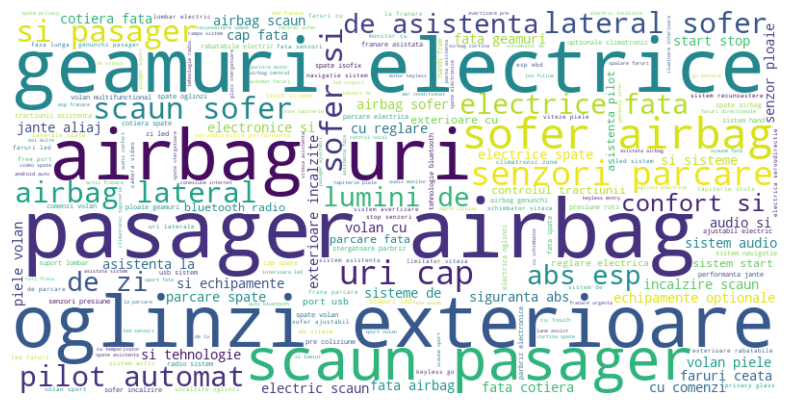
\includegraphics[width=\linewidth]{images/priceprediction/data/wordcloud.png}
    \caption{Descriptions Wordcloud}
    \label{fig:wordcloud}
\end{figure}


\subsubsection{Conclusion}
Our data analysis yielded valuable insights and a deep understanding of the dataset we scraped. We identified the key features that significantly impact car prices among our structured and numerical variables, validating our dataset by reflecting real-world market trends. Additionally, this analysis allowed us to preemptively identify potential issues, enabling us to focus more effectively on optimizing our model. These findings underscore the robustness of our dataset and provide a strong foundation for developing an accurate and reliable predictive model.

\chapter{Model}
In this chapter, we present our preprocessing steps and the incremental approach used to determine our final multimodal architecture. We conduct experiments with each model to demonstrate that the combined features enhance the accuracy of our final regression model.

\section{Preliminary}
Before starting the training process, we ensured our data was prepared and optimized for learning. This section details the preprocessing steps, data splitting strategy, and the metrics used throughout our model development.

\subsection{Preprocessing}
To enhance the learning process, we normalized our values using various tools from \textit{scikit-learn} \cite{scikit-learn} and \textit{pickle} \cite{pickle}. Scikit-learn, a Python module, offers valuable functions and classes for such tasks. We used pickle to save the fitted encoders and preprocessors for future inference.

We began by converting the boolean columns to integer values, followed by encoding the categorical columns. Initially, we attempted one-hot encoding for the categorical columns. One-hot encoding transforms each possible entry in the categorical columns into its own column with boolean values. However, this approach was suboptimal because our model's features became extremely sparse, with each manufacturer having five to thirty models. Instead, we opted for target encoding, which calculates the mean of the target variable where the encoded value is present.

Next, we normalized our values, which were now entirely numerical. Due to the differences in magnitude caused by our target encoding approach, it was crucial to use StandardScaler from scikit-learn to normalize the input values. StandardScaler calculates the mean and standard deviation for each feature, subtracts the mean from the current value, and divides the result by the standard deviation.

An unconventional experiment that proved beneficial for our task was scaling our target variable, the price. Although scaling the target variable is unusual in regression models, this approach improved the accuracy across all our models. We make sure to save the fitted scaler for future use, as we need the unscaled predictions for our users.

Descriptions do not require additional preprocessing, thanks to the formatting techniques applied during our formatting, cleaning, and analysis processes. These techniques, discussed earlier in the thesis, will be replicated during inference to ensure accurate results. The use of the tokenizer is detailed in \hyperref[sec:bert]{Section 4.3}. 

For training our FastVit model, we use its predefined preprocessing function with the \textit{is\_training} attribute set to \textit{True}. This function employs various traditional techniques, such as flipping, rotating and zooming, while also resizing the images to the model's required size of 256x256 pixels. This preprocessing step allows for a better generalization of the image encoder, making it more robust to the variety that we expect from user input. At inference, we are setting the attribute to \textit{False}, letting the predefined function do all the required preprocessing steps.

\subsection{Splitting Strategy}
In order for our experiments to be comparable, we adopted a pre-splitting strategy. Our splitting strategy and some preprocessing steps take place only one time, for all our experiments, therefore assuring that the results are comparable.

In our sparse dataset, it was crucial to distribute the data as evenly as possible. The distribution needed to match not only in terms of target value but also the features fed into the model. We aimed to avoid situations where a manufacturer, model, or other key features appeared only in one of the datasets. Initially, we attempted a clustering method using k-means, but after analyzing the distribution between our train and test datasets, we found it did not provide accurate separation.

Our final and most effective method was using a stratify key generated from multiple categorical columns:

\begin{lstlisting}
stratify_columns = ["manufacturer", "model", "fuel", "chassis", "is_automatic", "sold_by_company"]

for train_index, test_index in sss.split(df, df["stratify_key"]):
    train_set = df.iloc[train_index]
    test_set = df.iloc[test_index]
\end{lstlisting}

This approach resulted in a well-balanced split between the train and test datasets, as evidenced by the nearly identical distribution by price plot, scaled to the number of samples presented in \hyperref[fig:data-split]{Figure 4.1}. We used 80\% of our data for training and 20\% for testing.

\begin{figure}[ht]
    \centering
    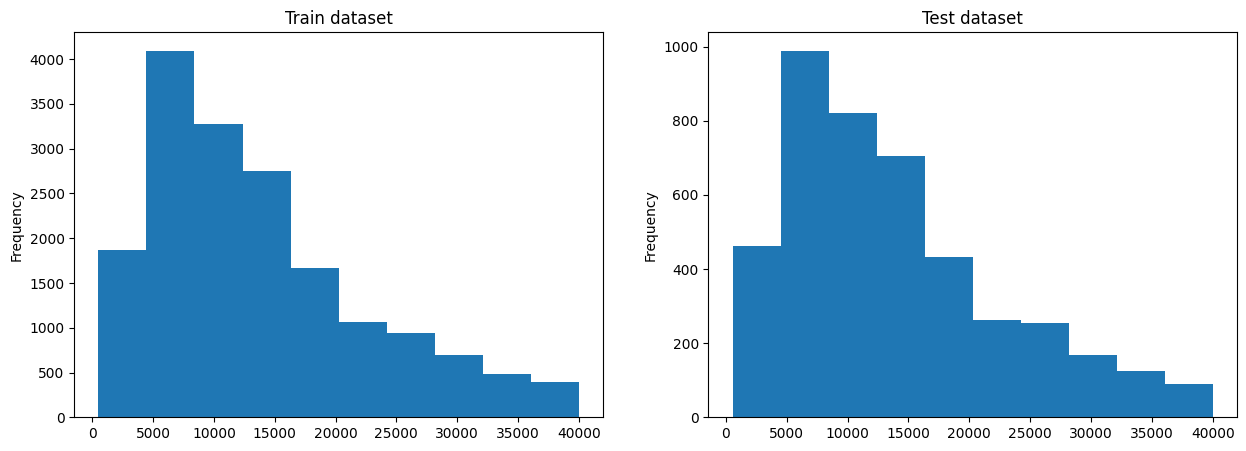
\includegraphics[width=\linewidth]{images/priceprediction/model/data_split.png}
    \caption{Train Test Data Split}
    \label{fig:data-split}
\end{figure}

\subsection{Metrics}

In this section, we describe three important metrics that we have used for evaluating our regression models: Mean Absolute Error (MAE), Mean Squared Error (MSE), and R-squared (\(R^2\)).

\subsubsection{Mean Absolute Error (MAE)}
\[ \text{MAE} = \frac{1}{n} \sum_{i=1}^{n} |y_i - \hat{y}_i| \]

\textbf{MAE}, also usually referred to as L1Loss, measures the average over the sum of absolute differences between the ground truth and predicted value

\textbf{Interpretation:}
\begin{itemize}
    \item A lower MAE indicates a better fit.
    \item MAE is less sensitive to outliers since it doesn't square the error compared to MSE, but it doesn't highlight large errors as much as MSE does.
\end{itemize}

\subsubsection{Mean Squared Error (MSE)}
\[ \text{MSE} = \frac{1}{n} \sum_{i=1}^{n} (y_i - \hat{y}_i)^2 \]

\textbf{MSE} also usually referred to as L2Loss, measures the average over the sum of the squared differences between the ground truth and predicted values.

\textbf{Interpretation:}
\begin{itemize}
    \item A lower MSE indicates a better fit.
    \item MSE gives a higher weight to large errors, thus being sensitive to outliers and penalizing them more than MAE.
\end{itemize}

\subsubsection{R-squared (\(R^2\))}
\[ R^2 = 1 - \frac{\sum_{i=1}^{n} (y_i - \hat{y}_i)^2}{\sum_{i=1}^{n} (y_i - \bar{y})^2} \]

\textbf{\(R^2\)} or \textit{coefficient of determination} provides valuable insights into how well the data fits the regression model. 

\textbf{Interpretation:}
\begin{itemize}
    \item \( R^2 \) ranges from 0 to 1, but sometimes can be even negative.
    \item A high \(R^2\) value means that the model explains the data it gets in a big proportion, meaning the data is representative for the task we are pursuing.
    \item A low \(R^2\) suggests that the data has more noise and less relevance to the model.
    \item Negative \( R^2 \) values can occur if the model performs worse than simply predicting the mean of the observed data.
\end{itemize}

\subsubsection{Summary}

These metrics together provide a comprehensive understanding of model performance from different perspectives.

\section{MLP - Structured Data}
Working with our self-scraped dataset, we lacked a baseline performance score. Our initial experiment involved creating a multilayer perceptron (MLP) as our baseline.

We utilized \textit{PyTorch} \cite{pytorch} as our deep learning framework. PyTorch simplifies the development of deep learning models by providing an accessible abstraction layer over the complex mathematical operations required. One of its key features is the utilization of CUDA (Compute Unified Device Architecture) cores for GPU acceleration, which significantly improves both training and inference computations. While \textit{TensorFlow} \cite{tensorflow} is a common alternative, we chose PyTorch due to its ease of use and support across all platforms, ensuring our code's reproducibility on various operating systems. In contrast, TensorFlow has support for CUDA only on Linux machines, which could limit its applicability.

The architecture of the Multilayer Perceptron (MLP) that yielded the best results after extensive fine-tuning comprises two fully connected (linear) hidden layers. The first hidden layer contains 128 neurons, while the second one contains 64 neurons.

ReLU activation functions are applied to each hidden layer to introduce non-linearity. Additionally, we use dropout with a rate of 0.2 on the second hidden layer to help prevent overfitting during the training phase.

For training this model, we will use the Adam optimization function with a learning rate of 1e-4 (0.0001). 

We use the L1Loss function as our loss metric. We chose L1Loss over the more commonly used L2Loss for regression tasks because our self-scraped dataset still contains some outliers that we do not want to unduly influence our model. This issue with outliers is evident in our final results presented in \hyperref[tab:best-results]{Table 4.1}, where the R-squared score is high, but the performance is not optimal.

During our training phase, we also implemented two important techniques: reducing the learning rate on a plateau and early stopping. Reducing the learning rate helps us to adjust the learning process when progress stalls, thereby improving convergence, and also allowing our model to focus on details later in the training session. Early stopping allows us to halt the training session early if overfitting or lack of further learning is detected, ensuring we save the best model from each training session.

\section{BERT - Text Encoder}
\label{sec:bert}
\textbf{B}idirectional \textbf{E}ncoder \textbf{R}epresentation from \textbf{T}ransformers (BERT) \cite{bert} is a transformer-based architecture, designed for encoding continuous pieces of text data. BERT builds on the transformer model introduced in the paper \textit{"Attention is All You Need"} \cite{attention}, which details the architecture's encoding and decoding components. BERT consists of multiple transformer encoder layers stacked on top of each other, similar to how GPT (Generative Pre-trained Transformer) is composed of stacked decoder layers. Its key features include faster processing speed, the ability to process multiple words simultaneously, and a deep understanding of context in a bidirectional manner.

For our problem, which involves inputs in Romanian, we will use a pre-trained version of BERT Base called Romanian BERT, introduced in the paper \textit{"The Birth of Romanian BERT"} \cite{dumitrescu-etal-2020-birth}. This model, based on BERT Base, contains 110 million trainable parameters and has been pre-trained on a 15GB corpus of Romanian text data.

Initially, we considered training a base BERT model from scratch. This idea stemmed from the unique language structure of our advertisement descriptions, which often contain numerous enumerations. However, we quickly realized that our data was insufficient for this approach, so we opted to use the pre-trained Romanian BERT model.

Throughout our training phase and during inference, we utilize the pre-trained tokenizer provided with the Romanian BERT model. The arguments passed to the tokenizer remain consistent. Although our data is already uncased, we add an extra layer of precaution by setting the \textit{do\_lower\_case} argument to \textit{True}. We instruct the tokenizer to add special tokens because we are particularly interested in the [CLS] token. Additionally, we set the maximum length accepted by BERT to 512, with both padding and truncation enabled. This maximum length is chosen because, after analyzing our descriptions, we found they often exceed this length, making truncation necessary.

\begin{lstlisting}
tokenizer = AutoTokenizer.from_pretrained("dumitrescustefan/bert-base-romanian-uncased-v1", do_lower_case=True, add_special_tokens=True, max_length=512, padding=True, truncation=True)
\end{lstlisting}

The fine-tuning phase of BERT involves two stages. The first stage trains BERT to understand the language, while the second stage fine-tunes it for our specific task, which is regression.

To train BERT to understand the language, we employed a self-supervised method known as masked language modeling (MLM). In this approach, 15\% of the tokens are masked, and BERT's task is to predict these missing words. For task-specific fine-tuning, we added two additional layers after the BERT embeddings. The first is a fully connected layer with 768 neurons, followed by a second layer with a single neuron representing our output. We use the [CLS] token embedding from BERT as the input to the first newly introduced layer, leveraging its comprehensive representation of the entire input.

\section{FastVit - Image Encoder}
FastVit \cite{fastvit} is a hybrid vision transformer architecture optimized for speed while maintaining high performance. It combines the strengths of both Vision Transformers (ViTs) and Convolutional Neural Networks (CNNs) to overcome their individual limitations. By integrating CNNs, FastVit enhances overall computation speed and improves local feature extraction and pattern recognition. The inclusion of Vision Transformers addresses the primary 
limitation of CNNs, which excel at finding fixed spatial relationships. By leveraging the attention mechanism from vision transformers, FastVit can understand the global context and capture relationships between different parts of an image.

For our task, we are using a pre-trained version of FastVit T8 for the same reason as with BERT: the lack of sufficient data. This pre-trained model has been trained on the IMAGENET1K dataset. We fine-tune the model for our regression task by adding the same layers as in our BERT approach. We also utilize the [CLS] token as the input to our newly introduced layers, utilizing its comprehensive representation.

\section{Multimodal Architecture}
Our final and best architecture for our multimodal model, showcased in \hyperref[fig:model-architecture]{Figure 4.2}, comprises fine-tuned versions of both BERT and FastVit, serving as text and image encoders, respectively. We utilize these models without the added fully connected layers, focusing on their pre-trained feature extraction capabilities for our regression task.

By using these fine-tuned encoders, we use their ability to extract essential features, which we then concatenate with our structured data, resulting in an input of 1546 features. In this setup, all layers of our encoders are frozen. However, a potential future enhancement could involve unfreezing these layers to enable full end-to-end fine-tuning throughout our architecture.

The concatenated input is then passed through the Multilayer Perceptron (MLP) shown in \autoref{lst:multimodal}, on which we apply ReLU activation functions and Dropout to introduce non-linearity and prevent overfitting, respectively. Additionally, early stopping is used to halt training if overfitting is detected or if there is no further improvement.

\begin{lstlisting}[label={lst:multimodal}]
model = nn.Sequential(
    nn.Linear(1546, 128),
    nn.ReLU(),
    nn.Dropout(0.2),
    nn.Linear(128, 64),
    nn.ReLU(),
    nn.Dropout(0.2),
    nn.Linear(64, 1)
)
\end{lstlisting}


\begin{figure}[ht]
    \centering
    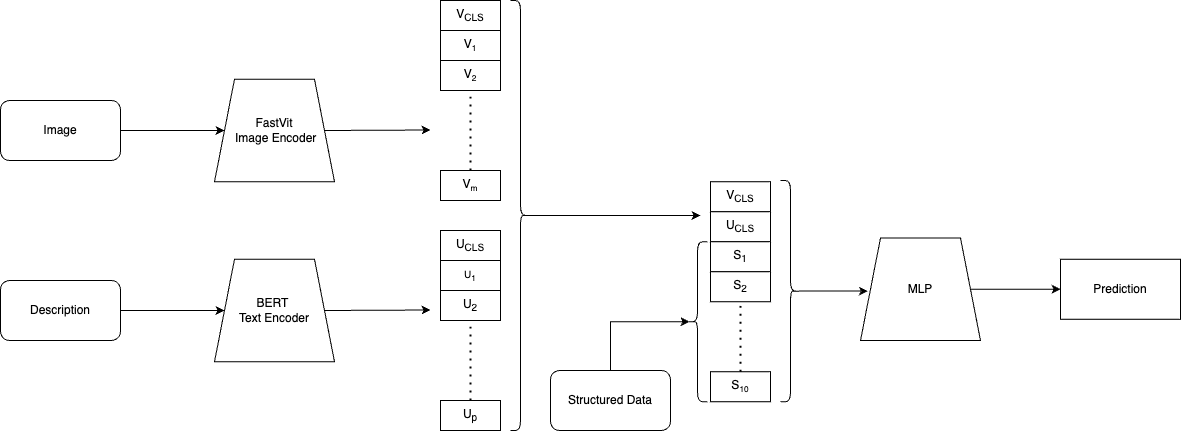
\includegraphics[width=\linewidth]{images/priceprediction/model/arch.png}
    \caption{Multi-modal architecture}
    \label{fig:model-architecture}
\end{figure}

In \hyperref[fig:multimodal-results]{Figure 4.3}, we present the training plots for our best multimodal model training session. The plots demonstrate a stable learning process. Notably, our test dataset initially performs better than the training set until epoch 130, where their performance converges. This suggests that the test dataset might be easier to predict, but given the small difference, we did not pursue further adjustments.

\begin{figure}[ht]
    \begin{subfigure}[b]{0.48\linewidth}
        \centering
        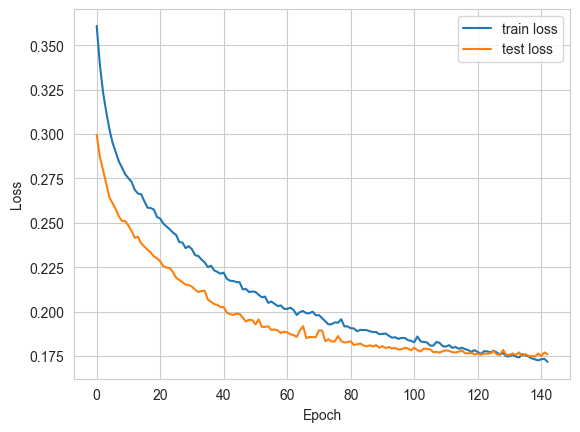
\includegraphics[width=\linewidth]{images/priceprediction/results/multimodal_loss.png}
        \caption{Loss (MAE)}
        \label{fig:multimodal-loss}
    \end{subfigure}
    \hfill
    \begin{subfigure}[b]{0.48\linewidth}
        \centering
        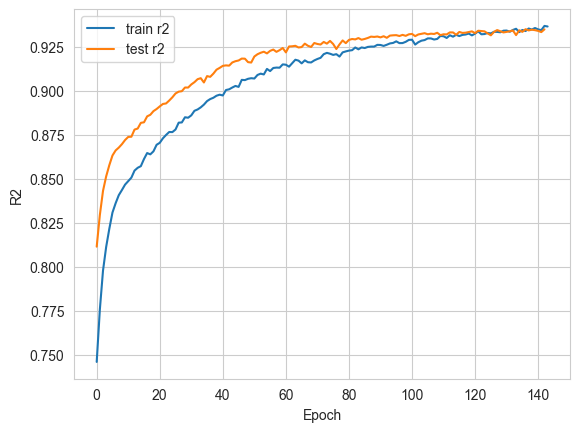
\includegraphics[width=\linewidth]{images/priceprediction/results/multimodal_r2.png}
        \caption{\(R^2\)}
        \label{fig:multimodal-r2}
    \end{subfigure}
    \caption{Multi-modal Training Plots}
    \label{fig:multimodal-results}
\end{figure}

\section{Results analysis}
In \hyperref[tab:best-results]{Table 4.1}, we present the results of our regression models, including both individual model outcomes and the final multimodal architecture. The results demonstrate that the most valuable features are found in the structured data, followed by descriptions and images. The best performance is observed in the multimodal architecture, validating our hypothesis that descriptions and images of advertisements provide valuable information for improving predictive accuracy.

\begin{table}[ht]
\centering
\begin{tabular}{lcccc}
    \textbf{Model} & \textbf{Environment} & \textbf{MAE} & \textbf{R2} \\ \hline
    \multirow{2}{*}{MLP} & Train & 1650 & 0.90 \\
                         & Test & 1698 & 0.895 \\ \hline
    \multirow{2}{*}{FastVit} & Train & 4007 & 0.623 \\
                             & Test & 4051 & 0.618 \\ \hline
    \multirow{2}{*}{BERT} & Train & 2427 & 0.85 \\
                          & Test & 2655 & 0.80 \\ \hline
    \multirow{2}{*}{Multimodal} & Train & \textbf{1522} & \textbf{0.936} \\
                                & Test & \textbf{1561} & \textbf{0.934} \\
\end{tabular}
\caption{Models best results}
\label{tab:best-results}
\end{table}

\chapter{Web Application}
To provide an accessible and user-friendly means of leveraging our vehicle price prediction model, we developed a web application designed for end-users. The primary functionality of this web application is to facilitate inference through an intuitive user interface and well-documented API endpoints.

\section{Architecture}
To ensure a scalable and maintainable solution, we designed our web application using a RESTful architecture. This approach allows for a clear separation of concerns between the frontend and backend, ensuring that the user interface (UI) remains independent of the underlying logic and data processing.

Representational State Transfer (REST) is an architectural style that uses standard HTTP methods to interact with resources, which are identified by URLs. Our backend exposes several RESTful endpoints that allow for interaction with the model and other functionalities of the application. These endpoints handle various operations, including data retrieval, model inference, payment and user authentication.

\section{Backend}
Considering our target clients, which include both our users and other businesses, we aimed to create a robust solution that could seamlessly integrate with any user interface. To achieve this, we developed a web application programming interface (API) that exposes our inference model, allowing clients to utilize it in various scenarios according to their needs.

\subsection{Tech Stack}
To ensure our backend could efficiently serve not only our client application but also external frontends, we chose \textit{FastAPI} \cite{fastapi} as our framework. FastAPI offers a multitude of advantages, including the automatic generation of interactive API documentation through Swagger, which provides comprehensive and easily navigable documentation for each endpoint when properly configured.

Our decision to remain within the Python ecosystem was driven by the need for seamless integration with machine learning packages. After considering Django, Flask, and FastAPI, we opted for FastAPI due to several compelling reasons:

\begin{itemize}
    \item \textbf{Performance}: The web, fundamentally based on HTTP requests, poses an I/O-bound heavy task for any web server. One of the standout features of FastAPI is its support for asynchronous programming, making it unique among Python web frameworks. This capability allows FastAPI to handle numerous simultaneous requests efficiently, reducing latency and improving overall performance. This, combined with its lightweight nature and the flexibility to choose all the other tools, makes it the most performant Python web framework available
    \item \textbf{Ease of use}: At its core, FastAPI addresses one of Python's long-standing challenges: the lack of static typing. Although type hints were introduced in Python 3.5, they do not provide the same level of static type enforcement as statically typed languages like C or Go. This often complicates the development process, making it more error-prone and less efficient. FastAPI, however, leverages type hints extensively, enhancing the developer experience significantly. By using type hints, FastAPI enables better code validation and error checking, akin to the benefits found in statically typed languages. Additionally, FastAPI offers an intuitive and modern approach to creating APIs through Python decorators. This makes defining endpoints straightforward and expressive, allowing us to build APIs with minimal boilerplate code.
    \item \textbf{Granularity and Flexibility}: Unlike Django, which is a comprehensive framework that includes built-in database adapters, an ORM, and migration tools, FastAPI provides developers with the freedom to choose their own tools and packages. This modularity allows for greater customization and flexibility, enabling developers to select the best components for their specific needs rather than being constrained by the framework’s built-in features.
    \item \textbf{Validation and Serialization}: Powered by \textit{Pydantic} \cite{pydantic}, FastAPI ensures robust data validation and serialization, reducing the likelihood of runtime errors and improving data integrity.
    \item \textbf{Interactive API Documentation}: One of the standout features of FastAPI is its automatic generation of interactive API documentation. Utilizing \textit{OpenAPI} \cite{openapi} and JSON Schema standards, FastAPI creates a detailed and interactive documentation interface with \textit{Swagger UI} \cite{swagger}.
\end{itemize}

\subsection{Architecture}
For our architecture, we adopted a modular approach. In line with the core principles of \textit{Clean Code} \cite{clean_code} by Robert C. Martin, which emphasize high readability, maintainability, and modularity, we chose to divide our logic into distinct modules. This approach not only enhances the clarity and organization of our codebase but also facilitates easier testing, debugging, and future enhancements. By breaking down the functionality into smaller, self-contained units, we ensure that each module adheres to the \textit{Single Responsibility Principle}, making the overall system more robust and adaptable to change.

\begin{itemize}
    \item \textbf{Schemas Module}: This module is responsible for configuring and defining all our API schemas, including request and response schemas for both successful operations and errors. It ensures that data structures are consistent and well-documented throughout the API.
    \item \textbf{APIs Module}: In this module, we define all our API endpoints and their associated documentation. It serves as the central hub for routing and handling API requests, ensuring that each endpoint is clearly documented and easily accessible.
    \item \textbf{Services Module}: This module contains the business logic and is invoked by our API endpoints. It acts as a bridge between user inputs and the repository module, processing the inputs and implementing the core functionalities of our application.
    \item \textbf{Repositories Module}: Called exclusively by our services, this module is responsible for all database interactions. It encapsulates the logic for data retrieval, storage, and manipulation, ensuring a clean separation of concerns.
    \item \textbf{S3 Module}: This data module is dedicated to configuring and managing our AWS S3 storage. It handles the download of processors and models at startup, providing essential resources for our application.
    \item \textbf{Auth Module}: This module handles the business logic for authentication. It manages user credentials, session management, and authorization processes, ensuring secure access to the application's features.
    \item \textbf{Models Module}: Utilizing an ORM (Object-Relational Mapping), this module is where our data models are defined and managed. It maps the database schema to Python objects, simplifying database operations.
    \item \textbf{Testing Module}: This module is dedicated to maintaining comprehensive tests, including both unit tests and integration tests. It helps us adhere to the single responsibility principle by isolating test configurations and ensuring that all aspects of the application are thoroughly tested.

\end{itemize}

The architecture is also presented in \hyperref[fig:backend-design]{Figure 5.1}.
\begin{figure}[ht]
    \centering
    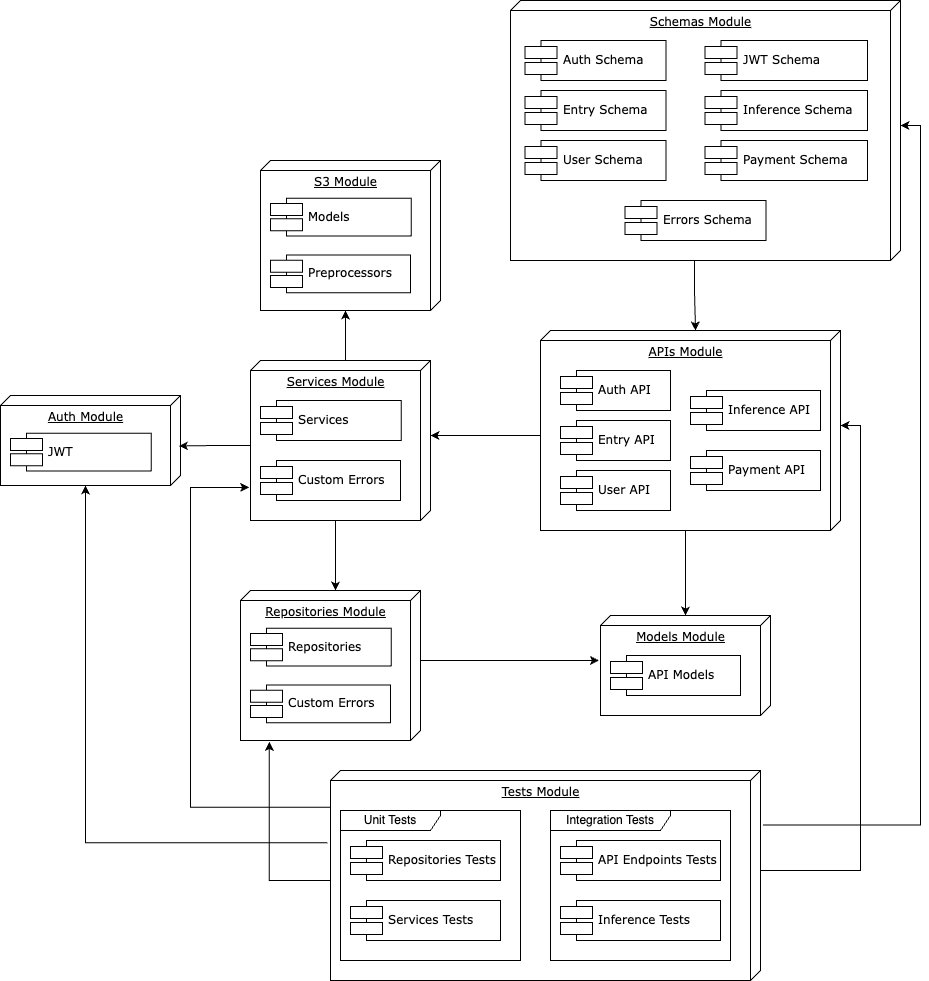
\includegraphics[width=0.8\linewidth]{images/webapp/backend/backend-modules.png}
    \caption{Backend Design}
    \label{fig:backend-design}
\end{figure}

For better scalability, we leveraged \textit{"Clean Code"} lessons further by creating abstractization layers for common tasks such as CRUD operations. This helps our app avoid code duplication and offers a better starting point for easy scalability in future updates.

In \hyperref[fig:backend-repositories]{Figure 5.2}, our abstractization is presented, along with our current services and repositories.

\begin{figure}[ht]
        \begin{subfigure}[b]{0.57\linewidth}
            \centering
            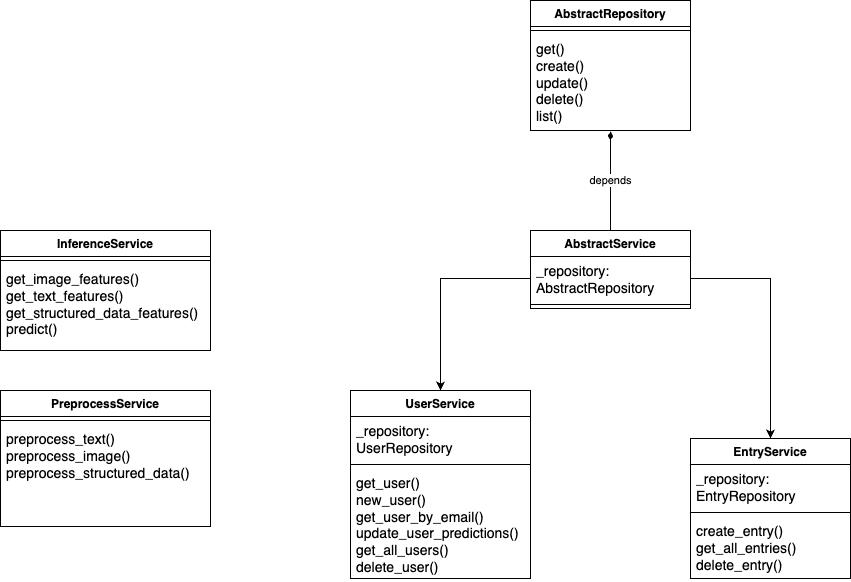
\includegraphics[width=\linewidth]{images/webapp/backend/services.png}
            \label{fig:backend-services}
        \end{subfigure}
        \hfill
        \begin{subfigure}[b]{0.43\linewidth}
            \centering
            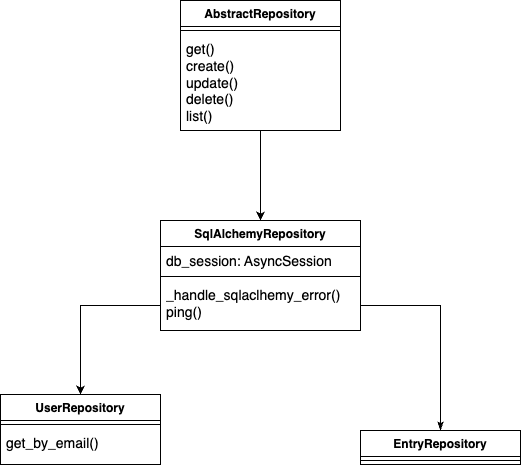
\includegraphics[width=\linewidth]{images/webapp/backend/repositories.png}
            \label{fig:backend-repositories}
        \end{subfigure}
        \caption{Services and Repositories}
        \label{fig:backend-design}
    \end{figure}

\subsection{Endpoints}
The \textit{RoCar API} exposes multiple endpoints, each with a distinct role, enabling seamless interaction with various functionalities of our application. All endpoints are prefixed with /api/v1 to ensure backward compatibility in future updates, preventing breaking changes. In this section, we will delve deeper into the specifics of each endpoint.

\subsubsection{Auth API}
The Auth API module manages the authentication processes, ensuring secure access to the application.
\begin{itemize}
\item \textbf{POST /login} - Validates user credentials and issues a JWT token upon successful authentication. This token is used for subsequent authenticated requests.
\item \textbf{POST /register} - Creates a new user account and returns a JWT token, enabling the user to access the application immediately after registration.
\end{itemize}

\subsubsection{User API}
The User API module provides endpoints for accessing user information.
\begin{itemize}
\item \textbf{GET /user/me} - Retrieves the current user's details, such as email, username, and the number of predictions remaining. This endpoint helps users verify their account information.
\end{itemize}

\subsubsection{Entry API}
The Entry API module allows users to manage their prediction entries.
\begin{itemize}
\item \textbf{GET /entry/all} - Fetches all previous predictions made by the user, allowing them to review their history and track their usage.
\item \textbf{DELETE /entry/{id}} - Deletes a specific prediction entry identified by its ID, giving users control over their data.
\item \textbf{POST /upload} - Uploads an image to the S3 bucket and returns its URL. This endpoint supports the integration of images into predictions, enhancing the model's accuracy.
\end{itemize}

\subsubsection{Payment API}
The Payment API module handles payment processes and interactions with the Stripe API \cite{stripe_api}. The entire payment integration flow can be visualised in \hyperref[fig:backend-stripe]{Figure 5.3}.

\begin{itemize}
\item \textbf{POST /create-checkout-session} - Initiates a checkout session with Stripe, providing a redirection link for the user to complete the payment. This ensures a secure and streamlined payment process.
\item \textbf{POST /webhook} - Listens for events from the Stripe API, such as successful or failed payments, and updates our system accordingly. This endpoint ensures that payment statuses are accurately reflected in our application.
\end{itemize}

\begin{figure}[ht]
    \centering
    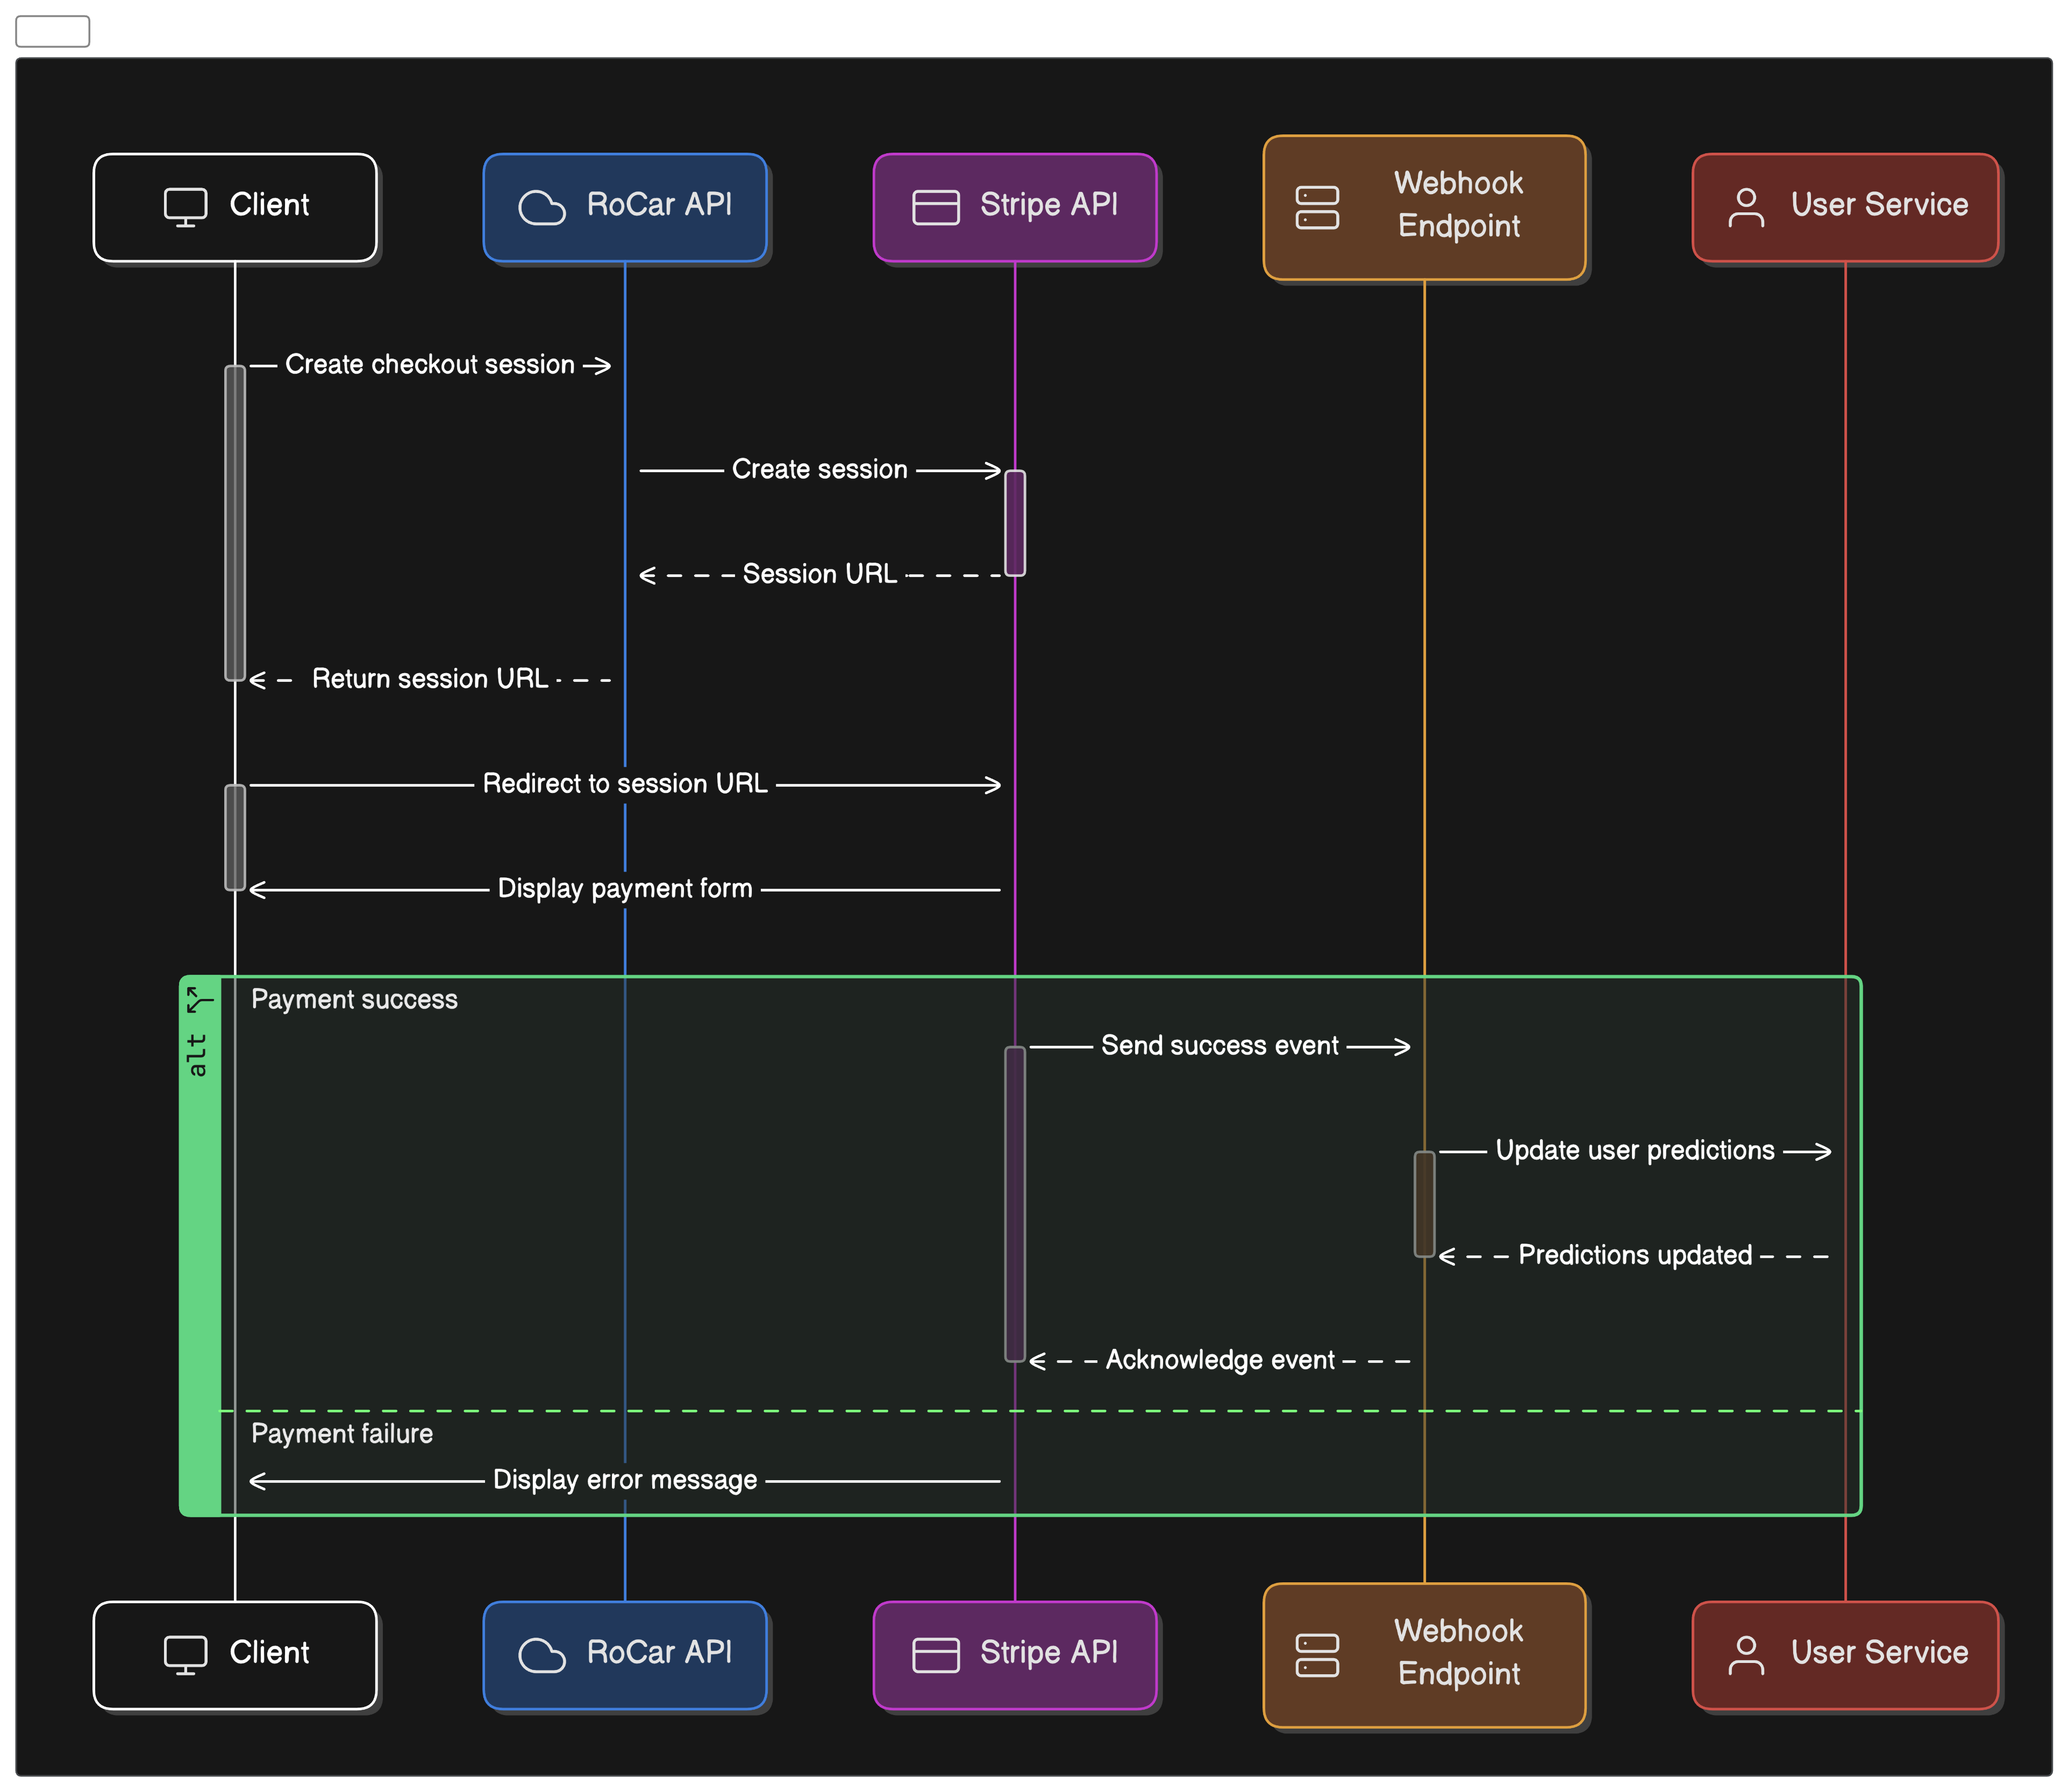
\includegraphics[width=0.7\linewidth]{images/webapp/backend/stripe.png}
    \caption{Stripe Flow}
    \label{fig:backend-stripe}
\end{figure}

\subsubsection{Inference API}
\begin{itemize}
    \item \textbf{POST /inference} - Gets the prediction of a car based on the inputs.
\end{itemize}

As our core functionality, we will showcase how it works in the next snippet.
\begin{lstlisting}
curl -X 'POST' \
  'http://127.0.0.1:8000/api/v1/inference' \
  -H 'accept: application/json' \
  -H 'Authorization: Bearer eyJhbGciOiJIUzI1...' \
  -H 'Content-Type: application/json' \
  -d '{
  "manufacturer": "audi",
  "model": "a3",
  "fuel": "gasoline",
  "chassis": "sedan",
  "sold_by": "company",
  "gearbox": "automatic",
  "km": 100000,
  "power": 160,
  "engine": 1984,
  "year": 2018,
  "description": "test description",
  "image_url": "https://thesis-s3.s3.eu-central-1.amazonaws.com/images/image.webp",
  "audio_and_technology": ["apple carplay", "infotainment system"],
  "comfort_and_optional_equipment": ["heated steering wheel"],
  "electronics_and_assistance_systems": ["rear sensors"],
  "performance": ["alloy wheels 17"],
  "safety": ["abs", "esp"]
}'

{
  "prediction": 15839
}
\end{lstlisting}

\subsection{RDBMS}
To efficiently manage and organize the data throughout our application, we selected a robust relational database management system (RDBMS) stack. The chosen stack comprises \textit{PostgreSQL} \cite{postgresql} as the database, \textit{SQLAlchemy} \cite{sqlalchemy} as the Object-Relational Mapping (ORM) library, \textit{Alembic} \cite{alembic} for database migrations, and \textit{Amazon S3} \cite{amazon_s3} for image storage.

\begin{itemize}
    \item \textbf{PostgreSQL}: We opted for PostgreSQL as our database due to its open-source nature, strong community support, and advanced features. PostgreSQL is known for its reliability, scalability, and compliance with SQL standards.
    \item \textbf{SQLAlchemy}: To interact with the PostgreSQL database, we used SQLAlchemy, a powerful ORM library for the Python ecosystem. SQLAlchemy simplifies database operations by allowing us to interact with the database using Python objects instead of writing raw SQL queries. This enhances code readability and maintainability, enabling more efficient development processes.
    \item \textbf{Alembic}: Database schema changes are a common requirement during the development lifecycle. Alembic, a database migration tool, integrates seamlessly with SQLAlchemy to manage database schema changes. It allows for the automatic generation of migration scripts, ensuring that database schema updates are consistent and easily reproducible across different environments.
    \item \textbf{Amazon S3}: For storing images associated with car advertisements, we utilized Amazon S3. S3 provides a highly scalable and durable storage solution, capable of handling large volumes of image data. Its integration with our RDBMS stack ensures that images are securely stored and easily accessible for display within our application.
\end{itemize}

Implementing the RDBMS stack involved several key steps to ensure seamless integration and optimal performance:

\begin{itemize}
    \item \textbf{Database Schema Design}: We designed a normalized database schema in PostgreSQL, focusing on minimizing redundancy and ensuring data integrity. Our current database consists of only two tables, one for the user and one for entry, connected by a one-to-many relationship. Although it is a really simple schema at the time of writing, it can be easily scaled by adapting our models module and running the migrations.
    \item \textbf{ORM Configuration}: SQLAlchemy was configured to map the database tables to Python classes present in our Models module, enabling object-oriented interaction with the database.
    \item \textbf{Migration Management}: Alembic was used to manage database migrations, ensuring that schema changes were consistently applied across all development, testing, and production environments. Automated migration scripts were generated to handle schema updates, reducing the risk of manual errors.
    \item \textbf{Image Storage Integration}: Amazon S3 was integrated into the stack for image storage. Metadata for images, such as URLs, were stored in the PostgreSQL database, while the actual image files were securely stored in S3. This separation allows for efficient data management and retrieval.
\end{itemize}

\subsection{Testing}
Testing is a crucial aspect of the development lifecycle, especially for a production-ready application. Our focus was not only on creating tests that pass but also on simulating a real production environment. This approach ensures that any changes we make do not break existing functionality, thereby maintaining the stability and reliability of our application.

We utilized the power of \textit{pytest} \cite{pytest} and \textit{pytest-asyncio} \cite{pytest_asyncio} for their easy configuration, effective mocking capabilities, and fast testing speeds. Our testing strategy includes both unit tests and integration tests to comprehensively validate our application.

\subsubsection{Unit tests}
In our unit tests, we concentrated on testing the core functionality of our services and repositories. Mocking was our primary method for handling external dependencies, allowing us to isolate and test individual components effectively.

\begin{itemize}
    \item \textbf{Focus}: The primary focus was on ensuring that each module behaves as expected in isolation.
    \item \textbf{Coverage}: Our unit tests achieve a coverage of 99\%, with all 30 tests passing consistently.
    \item \textbf{Tools}: We utilized mocking extensively to simulate external services and dependencies, ensuring that tests are self-contained and reliable.
\end{itemize}

\subsubsection{Integration tests}
To simulate a real production environment during testing, we set up a dedicated database before running integration tests. This setup was achieved using a custom Docker Compose configuration file and a custom Docker image for our application.

For an easier testing process, we create a custom script that does all the steps for us, from starting the test database, to cleaning pycache and saving the coverage for us.

The script is made with the task runner \textit{poethepoet} \cite{poethepoet}, that has it's config inside the pyproject.toml file from our virtual environment managed with \textit{poetry} \cite{poetry}.

We used this tool for various repetead cli commands, for an easier development experience:

\begin{lstlisting}[language={}]
CONFIGURED TASKS
  clean                    Clean up the project
  clean_pycache            Clean up the project of all __pycache__ folders
  unit_test                Clean artifacts and run unittests
    --cov-report           Generate coverage html or xml report
  build_image              Build docker image
    --tag                  Tag of the docker image [default: latest]
  start_app                Start the app
  stop_app                 Stop the app
  integration_test         Run API tests in a new environment
    --cov-report           Generate coverage html or xml report
  create_migration         Create migration
  upgrade_schema           Upgrade database schema
  downgrade_schema         Downgrade database schema
\end{lstlisting}

\begin{itemize}
    \item \textbf{Environment Simulation}: By spinning up a database and other necessary services, we created an environment that closely mimics production, allowing us to test the interactions between various components in a real world scenario.
    \item \textbf{Isolation}: Each test is designed to run independently, with no dependencies on other tests. This isolation ensures that tests do not pass or fail due to side effects from other tests.
    \item \textbf{Coverage}: Our integration tests achieve a coverage of 99\%, with all 32 tests passing consistently.
    \item \textbf{Tools}: We used Docker and Docker Compose to manage the setup and teardown of the testing environment, ensuring consistency and repeatability.
\end{itemize}

By employing a comprehensive testing strategy that includes both unit and integration tests, we ensured that our application is robust, reliable, and ready for production. This approach helps us maintain high code quality and quickly identify and resolve issues, providing confidence in the stability of our system.

\subsection{Deployment}
For our API we employed an automatic deployment, managed with \textit{Github Actions} \cite{github_actions}. We created rules, and jobs that check our code quality, runs tests, and sends a signal to \textit{Render} \cite{render} (our deployment platform) to pull the changes and run the deployment.

On Render, our app is deployed by it taking our custom docker image from our github repository. There we have set up a multi staged docker image, that has 3 stages.

\begin{itemize}
    \item \textbf{Base}: In the base stage we make sure poetry is installed in our container.
    \item \textbf{Development stage}: This stage is for developers, any contributor can pull the repository and run this stage step for an easy development without any additional setup.
    \item \textbf{Prepare Production Stage}: For our production environment, we aim to be as close to the metal as possible to enhance security. Therefore, this step removes Poetry and installs the dependencies using pip. We use the python:3.12-slim image to minimize security risks associated with larger base images.
    \item \textbf{Production Stage}: This is the final stage, where we utilize the dependencies installed in the previous step and start our server. A custom bash script is executed to first run migrations and then start the server.
\end{itemize}

An essential aspect of our deployment, and indeed across all our environments, is the loading process for our models and preprocessors. Before starting the server, we verify if the latest model and preprocessors are already present on the server. If they are, we proceed with the server startup. If not, we initiate the download process from our manually maintained S3 bucket. This workflow is consistently applied in local development, \textit{Docker} \cite{docker} development, testing environments, and production environments.


Our Github Actions setup is visually illustrated in \hyperref[fig:backend-cicd]{Figure 5.4}.
\begin{figure}[ht]
    \centering
    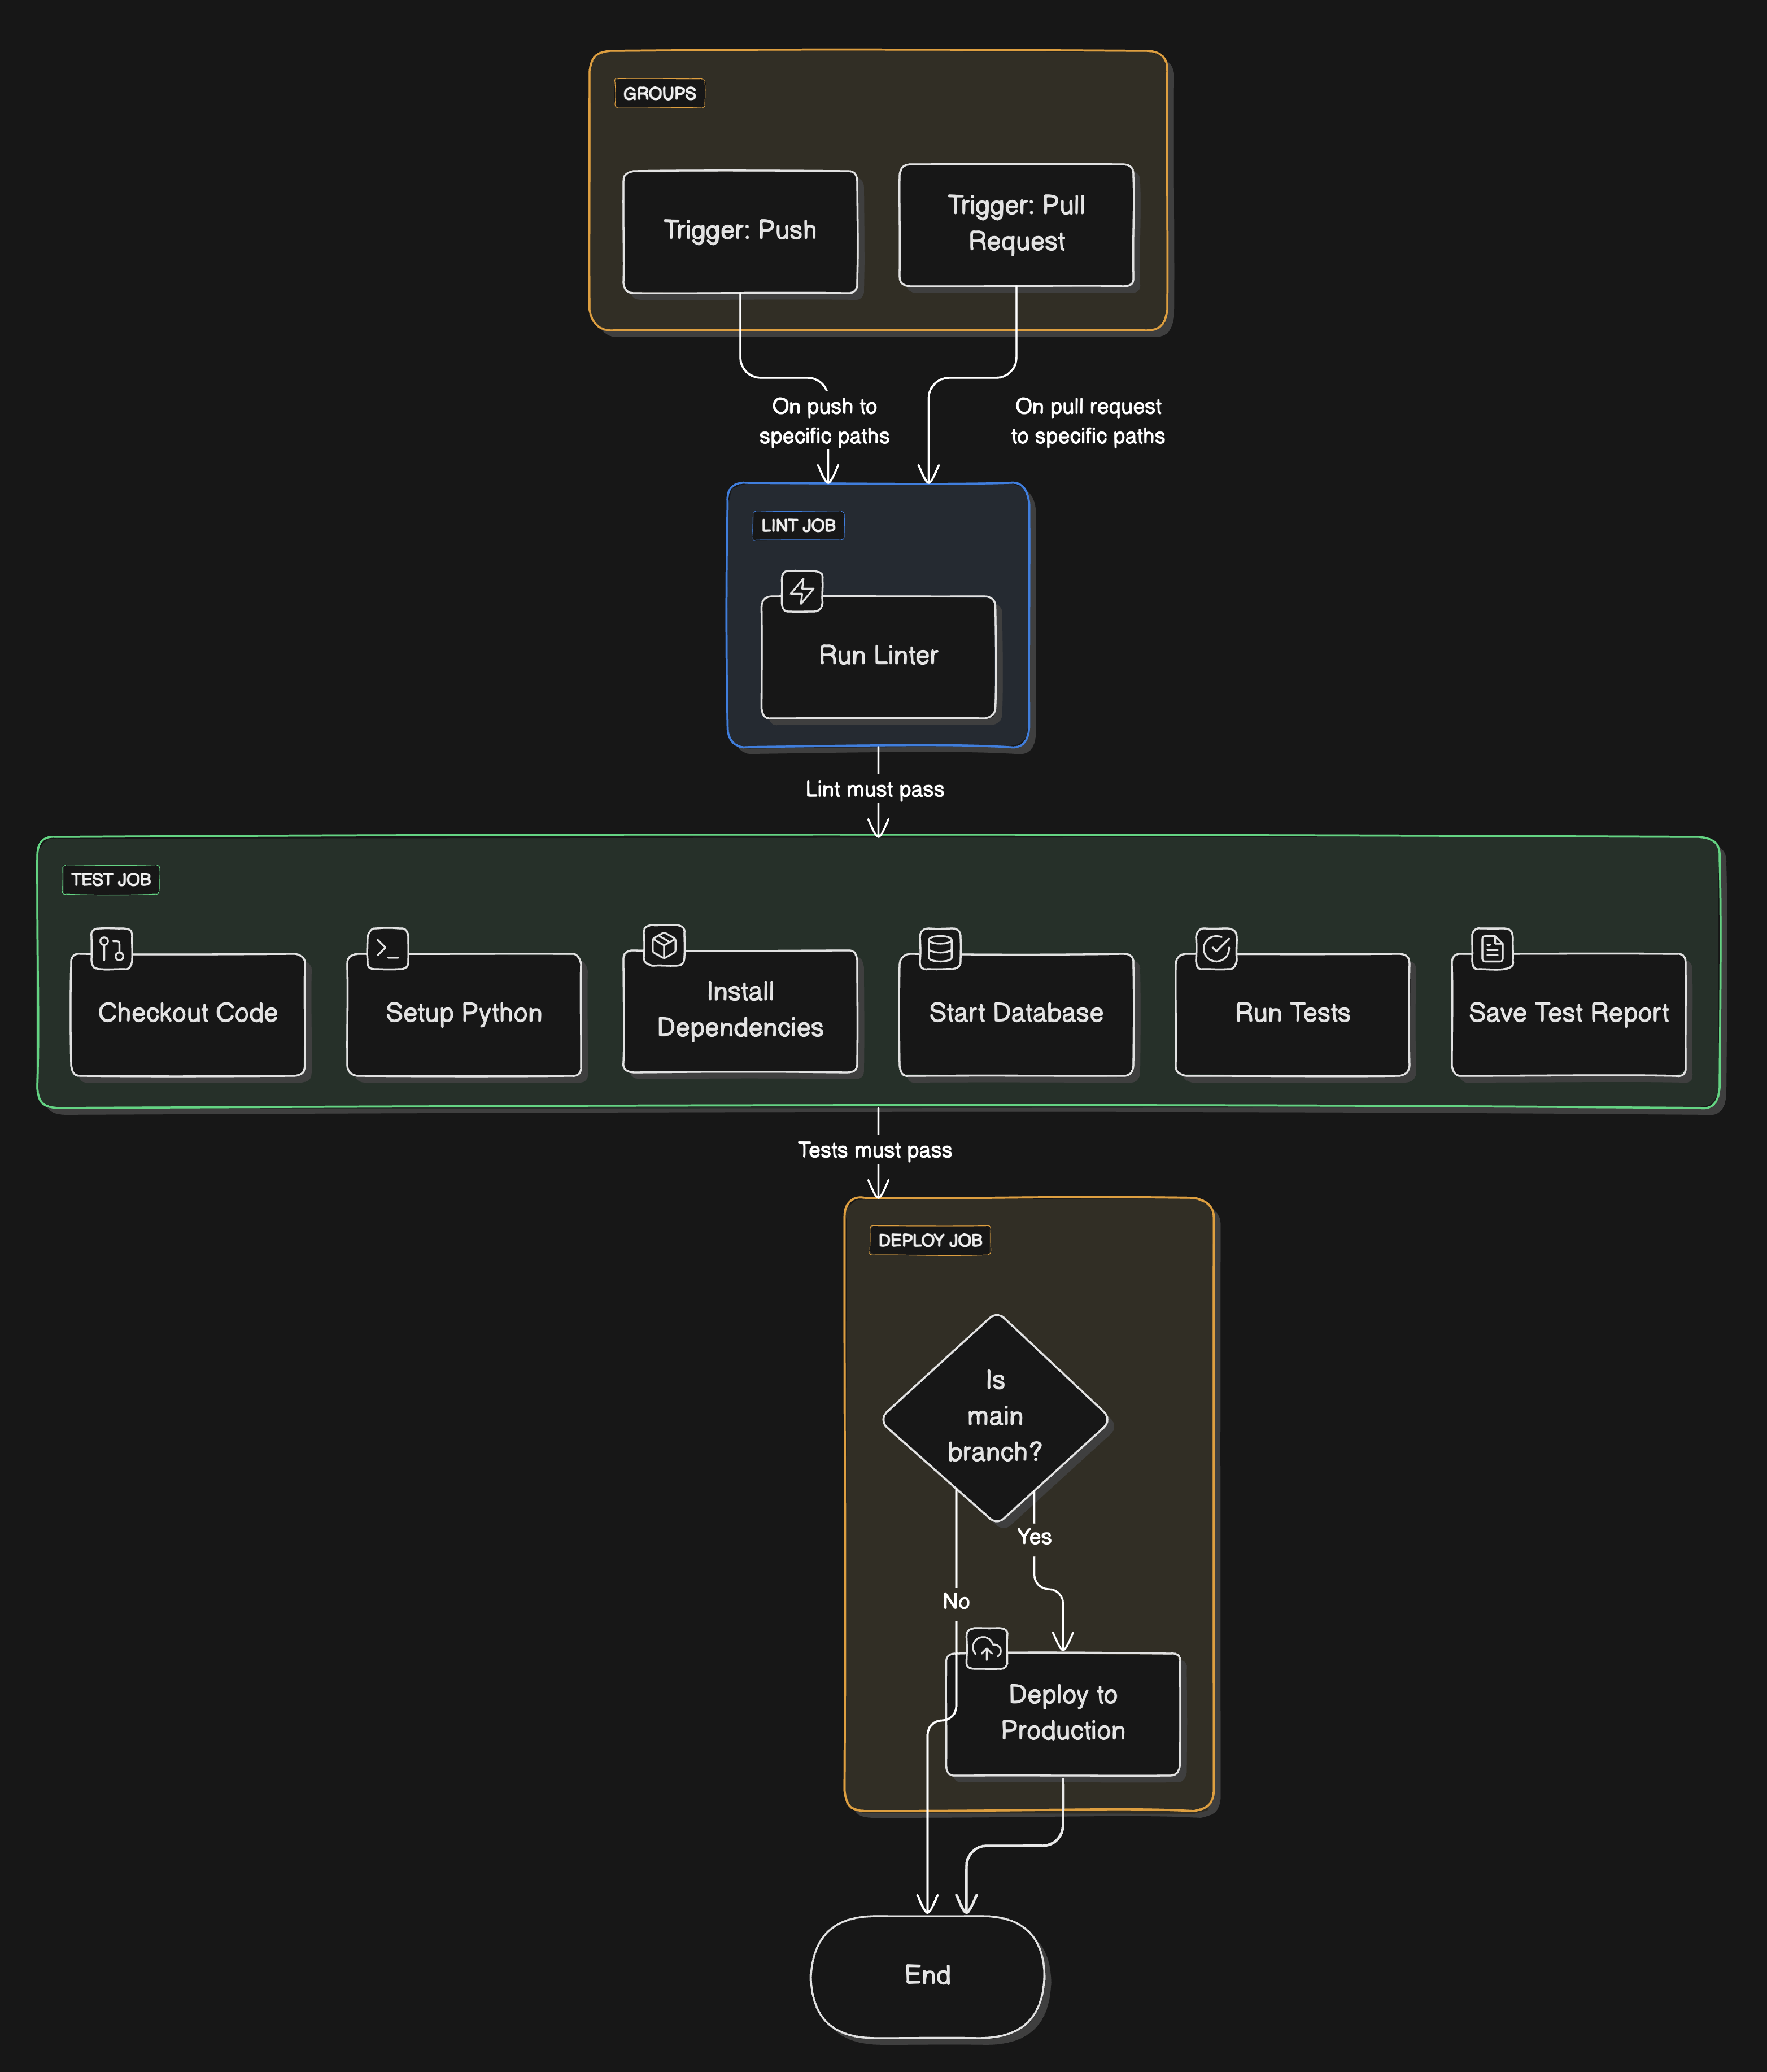
\includegraphics[width=\linewidth]{images/webapp/backend/cicd.png}
    \caption{Github Actions Pipeline}
    \label{fig:backend-cicd}
\end{figure}


\subsection{Environments}
All secrets within our app are securely stored in ignored .env files in the local environment, in GitHub secrets within our remote repository, and in Render and Vercel secrets for our deployment services. This ensures that sensitive information, such as our secret key for generating JWTs, remains protected. We maintain separate .env files for each stage: testing, development, and production, that are injected accordingly using our custom cli commands.

\section{Frontend}
In addition to the logic and functionality provided by our API, we recognized the need to make our model accessible to non-technical users. To achieve this, we developed a minimal, responsive user interface that ensures ease of use across all devices. This intuitive interface empowers users of all technical backgrounds to seamlessly interact with our model, providing a streamlined and user-friendly experience.

\subsection{Tech Stack}
Our tech stack features \textit{Next.js} \cite{nextjs}, a comprehensive framework built on React. Next.js provides significant value out of the box, including features such as caching, server-side rendering (SSR), and support for React Server Components. These capabilities ensure fast, dynamic, and SEO-friendly web applications.

In terms of our UI library, we opted for \textit{Shadcn} \cite{shadcn}. Shadcn is a headless component library that allows for complete control over styles. It leverages \textit{Tailwind CSS} \cite{tailwind_css}, providing a highly customizable and efficient styling solution.

\subsection{Pages}
The user interface comprehends six pages:

\begin{itemize}
    \item \textbf{Login page}: The page where users log in with their existing accounts.
    \item \textbf{Register page}: The page where users create accounts and then are redirected to their dashboard.
    \item \textbf{Landing page}: A public route landing page where we market our application.
    \item \textbf{Pricing page}: A public route pricing page, where users can see our pricing models. When not authenticated, they can still see the page, but if they want to buy one of our packages, they are redirected to the login page.
    \item \textbf{Dashboard page}: A private route page where authenticated users can see their old predictions made within our app.
    \item \textbf{Prediction page}: A private route page where the users are prompted with a rather big form where they insert the necessary information for the prediction.
\end{itemize}

\subsection{Deployment}
The deployment platform for our user interface is \textit{Vercel} \cite{vercel}. We connected the Vercel project to our repository, and each time a change is seen in the main branch in our frontend directory, the automatic deployment process starts. Vercel offers zero downtime deployment out of the box, an important requirement for a production ready application.

\chapter{Conclusion and Future Work}

\section{Future Work}

Although our goal was to create a fully-fledged framework for our concept, we encountered several challenges that prevented us from reaching this objective fully. Despite these hurdles, we believe we have developed a robust Minimum Viable Product (MVP) that can be easily scaled and enhanced, thanks to our strategic architectural decisions.

In the following sections, we will delve deeper into the key areas for future development:

\subsection{Dataset}

Our experiments demonstrated the importance of descriptions and images in our regression model. However, the primary limitation was our self-scraped dataset. While it sufficed for our initial analysis and experiments, it is not yet suitable for handling edge cases in a production environment.

Our goal is to create a more comprehensive dataset. We plan to achieve this by refining our scraping model, supported by manual effort at times, to ensure data quality and completeness. We envision providing more structured data parameters, along with high-quality images of both the exterior and interior of vehicles from various angles and possibly a standardized description format. We believe this enhancement will significantly improve our model's performance.


\subsection{API}

Currently, our app offers a minimal API for our customers. There are several additional aspects that are typically expected in a finalized product, which we aim to incorporate in future iterations:

\begin{itemize}
\item \textbf{Statistics}: Leveraging our extensive dataset, we can offer users detailed statistics on market trends and provide insights into their previous predictions made within the app. This feature will add significant value by helping users make informed decisions.
\item \textbf{Performance}: At present, the app is hosted on a single server, which could quickly become a bottleneck due to the resource-intensive nature of our models. Implementing a scalable deployment strategy will ensure a smoother and more reliable user experience.
\item \textbf{Multi-Country Support}: While our initial focus has been on the Romanian market, the challenges we address are prevalent in multiple countries. Expanding our support to include other markets will broaden our user base and enhance the app's utility.
\end{itemize}

\subsection{Frontend}

Although we have developed a fully functional UI for our users, there is considerable room for improvement. The current design is minimal and functional but lacks visual appeal. In today's web landscape, a more engaging and aesthetically pleasing design is crucial. Enhancing the UI to be more visually attractive will improve user engagement and satisfaction.

\section{Conclusion}

This thesis presents \textit{RoCar}, a web application designed to empower buyers in the complex Romanian second-hand car market. Utilizing a comprehensive, self-scraped dataset and employing a multimodal approach incorporating textual and visual data analysis, \textit{RoCar} significantly enhances the accuracy and depth of car price predictions compared to existing tools.

The development of \textit{RoCar} highlighted the critical importance and inherent challenges of working with self-scraped data. The iterative process of data collection, cleaning, and formatting demanded significant effort and expertise, underscoring the need for meticulous data preparation in machine learning applications.

In conclusion, predicting the price of a second-hand car is still a complex challenge due to the multiple factors involved. However, in this thesis, we presented metrics and techniques that we hope will pave the way to future improvements and better results in the automotive sector of machine learning.



\printbibliography[heading=bibintoc]

\end{document}